% !TeX root = main.tex

\documentclass[10pt,aspectratio=169,dvipsnames]{beamer} % sets document type, default font size, slide aspect ratio, and loads color names
\usetheme[color/block=transparent]{metropolis} % sets the theme of the document

\usepackage[absolute,overlay]{textpos} % allows absolute positioning of text
\usepackage{booktabs} % enhances quality of tables
\usepackage[utf8]{inputenc} % allows input encoding in UTF-8
\usepackage{tikz} % used for creating vector graphics
\usetikzlibrary{arrows.meta} % loads additional arrow types
\usepackage[europeanresistors,americaninductors]{circuitikz} % for drawing electrical circuits
\usepackage[scale=2]{ccicons} % loads Creative Commons icons
\usepackage[official]{eurosym} % loads the official symbol for the Euro
\usepackage{hyperref} % allows creating hyperlinks in the document

\newcommand{\ra}[1]{\renewcommand{\arraystretch}{#1}} % creates command to adjust spacing between rows
\newcommand{\hrefc}[2]{\href{#1}{\bf\color{blue}{\underline{#2}}}} % defines command for underlined, blue hyperlink
\newcommand{\urlc}[1]{\hrefc{#1}{#1}} % defines command for URL hyperlink

\newcommand{\R}{\mathbb{R}} % creates a shortcut for typing real numbers symbol
\newcommand{\ubar}[1]{\text{\b{$#1$}}} % defines a command for underlined text

\xdefinecolor{TUred}{RGB}{197,14,31} % defines a new color TUred
\setbeamerfont{alerted text}{series=\bfseries} % sets the font of alerted text to bold
\setbeamercolor{alerted text}{fg=TUred} % sets the color of alerted text to TUred
\setbeamercolor{background canvas}{bg=white} % sets the background color to white
\setbeamercolor{frametitle}{bg=lightgray!40, fg=TUred} % sets the background color of the frame title to light gray and text color to TUred
\setbeamercolor{title}{fg=TUred} % sets the color of the title to TUred

\addtobeamertemplate{frametitle}{}{% adds image to every frame title
  \begin{textblock*}{100mm}(1.01\textwidth,2pt)
    
\includegraphics[width=1.5cm]{images/TUB.png}
    \end{textblock*}}

\def\l{\lambda} % defines a shortcut for lambda symbol
\def\m{\mu} % defines a shortcut for mu symbol
\def\d{\partial} % defines a shortcut for partial symbol
\def\cL{\mathcal{L}} % defines a shortcut for caligraphic L symbol
\def\co{CO${}_2$} % defines a shortcut for CO2 symbol
\def\el{${}_{el}$} % defines a subscript for el
\def\th{${}_{th}$} % defines a subscript for th
\def\gas{${}_{gas}$} % defines a subscript for gas

\setbeamercolor{framesource}{fg=gray} % sets color of framesource to gray
\setbeamerfont{framesource}{size=\tiny} % sets font size of framesource to tiny
\newcommand{\source}[1]{% creates command for inserting a source footnote
\begin{textblock*}{5cm}(10.5cm,8.35cm)
    \begin{beamercolorbox}[ht=0.5cm,right]{framesource}
        \usebeamerfont{framesource}\usebeamercolor[fg]{framesource} {#1}
    \end{beamercolorbox}
\end{textblock*}}

\graphicspath{{../results/}} % sets the path where graphics can be found
\DeclareGraphicsExtensions{.pdf,.jpeg,.png,.jpg} % defines the types of graphic files that can be used

\def\goat#1{{\scriptsize\color{green}{[#1]}}} % defines a command for green, scriptsize text

\let\olditem\item % saves the old item command
\renewcommand{\item}{\olditem\vspace{5pt}} % redefines the item command to add space after each item


\title{On space-time load-shifting flexibility for data centers \\ 
      \& 24/7 carbon-free electricity procurement}

%\subtitle{---}
\author{
  Iegor Riepin, Tom Brown\\
  \hrefc{https://www.tu.berlin/en/ensys}{Department of Digital Transformation in Energy Systems}, TU Berlin
  }

\date{23 June 2023}

\titlegraphic{%
  \vspace{0cm}
  \hspace{10.7cm}
    
\includegraphics[trim=0 0cm 0 0cm,height=1.2cm,clip=true]{images/TUB.png}
  \vspace{5.1cm}
  \\ \faGithub \href{https://github.com/PyPSA/247-cfe}{ Open code}
  \\ \faShareAlt \href{https://pypsa.org/}{ PyPSA community}
  }

\begin{document}

\maketitle

\begin{frame}
  \frametitle{Acknowledgements}

  \begin{itemize}
    \item {\bf Funding:} This study was supported by a grant from Google, Inc. 
    \item {\bf Acknowledgements:} The authors thank members of the Google energy markets and policy team 
    for their feedback and inputs on earlier drafts of this study. 
    We also thank the \hrefc{https://pypsa.org/}{PyPSA team} and many contributors to the open-source 
    energy system modelling ecosystem used for this study (see: \hrefc{https://github.com/PyPSA/PyPSA}{github.com/PyPSA}).
    Warm thanks to Fabian~Hofmann for making complex optimization simpler with \hrefc{https://linopy.readthedocs.io/}{linopy}. 
    \item 
    {\bf Copyright} Unless otherwise stated, graphics and text are Copyright \copyright Tom Brown and Iegor Riepin, 2023.
    Graphics and text for which no other attribution are given are licensed under a 
    \href{https://creativecommons.org/licenses/by/4.0/}{CC BY 4.0}.  {\footnotesize \ccby} 
    \item The content of this study, including any errors or omissions, are the responsibility
    of the authors alone.
  \end{itemize}

\end{frame}


\begin{frame}{Summary of key findings}

  \centering
  {\small

  \noindent\fbox{%
  \parbox{\textwidth}{%
    \begin{enumerate}

    % \item 24/7~carbon-free energy (CFE) procurement leads to lower emissions for both the buyer and the system,
    %   as well as reducing the needs for flexibility in the rest of the system.  

    % \item Reaching CFE for 90-95\% of the time can be done with only a small cost premium compared to annually matching 
    % 100\% renewable energy. 90-95\% CFE can be met by supplementing wind and solar with battery storage.

    % \item Reaching 100\% CFE target is possible but costly with existing renewable 
    % and storage technologies, with costs increasing rapidly above 95\%.
    
    % \item 100\% CFE target could have a much smaller cost premium if long duration storage or 
    % clean dispatchable technologies like advanced geothermal are available.
    
    % \item 24/7~CFE procurement would create an early market for the advanced technologies,
    % stimulating innovation and learning from which the whole electricity system would benefit.
    
    \item Space-time load-shifting flexibility facilitates economically efficient redistribution of data center loads.
    \item This effect comes with a ... and reduction of renewable energy curtailment.
    \item Flexible operation helps achieving a 24/7 hourly matching of electricity demand with clean energy with smaller resources. This can facilitate more data center operators and other flexible electricity buyers to join the 24/7~CFE efforts. 
    \item Space-time load management can enable achieving 24/7~CFE procurement goals simpler for other companies who do not have such flexibility options. 
    \item on LDES? on emission reduction with lower cost?

  \end{enumerate}
  }}
  }
  
\end{frame}



\begin{frame}
  \frametitle{Table of Contents}
  \setbeamertemplate{section in toc}[sections numbered]
  \tableofcontents[hideallsubsections]
\end{frame}


%----------------------------------------
%----------------------------------------

\section{Introduction}


\begin{frame}{Introduction}

  \centering
    \begin{itemize}
    \item Climate change is driving a global effort to rapidly decarbonise 
    electricity systems across the globe. 
    Many public and private energy buyers have joined this effort 
    by purchasing certificates for renewable energy or
    by procuring renewable energy directly with Power Purchase Agreements (PPAs).
    \item Such \alert{voluntary commitments accelerate the deployment of renewable 
    capacity} above the policy requirements in the countries and jurisdictions
    where these companies operate, facilitating faster
    transformation of electricity markets.
    \item Additionally, many early actors in the field have paved the way for others to follow 
    \hrefc{https://www.gstatic.com/gumdrop/sustainability/247-carbon-free-energy.pdf}{by 
    developing methods and establishing standard contracts} for clean energy procurement.
    \end{itemize}
  
\end{frame}



\begin{frame}{Introduction}

  \begin{columns}[T]
    \begin{column}{6cm}
      \begin{itemize}
        \item   PPAs typically are typically used for renewable energy to match generation 
        and consumption on average over a year.
        \item For example, more than 370 members of the \href{https://www.there100.org/}{RE100} group have committed to purchasing enough renewable energy to match
        \alert{100\% of their electricity consumption on an annual basis}.
      \end{itemize}
    \end{column}

  \begin{column}{10cm}
      \centering
      
      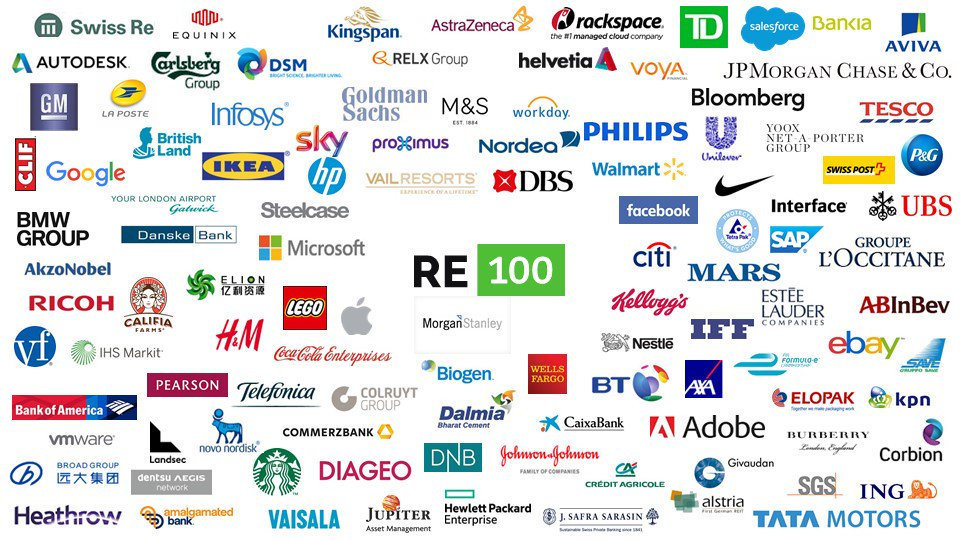
\includegraphics[width=10cm]{images/100re-companies.jpg}
      \vspace{.1cm}
      {\footnotesize
      More than 370 companies have joined \hrefc{https://www.there100.org/}{RE100}
      }
    \end{column}
    \end{columns}

    \source{source: \href{https://www.there100.org/}{RE100}}
\end{frame}
  


\begin{frame}{Introduction}
  
    \begin{itemize}
    \item However, electricity buyers that commit to 100\% annual matching 
    from renewable energy sources still face times when generation 
    from wind and solar generators is not sufficient to match 
    the companies’ electricity demand. 
    \item Thus, although buyers match their demand on a \alert{yearly} basis with 
    renewable energy, on an \alert{hourly} basis they still have hours 
    when they have to rely on carbon-emitting technologies available 
    on the local market, such as coal and gas-fired power plants.
    \end{itemize}

  \centering
  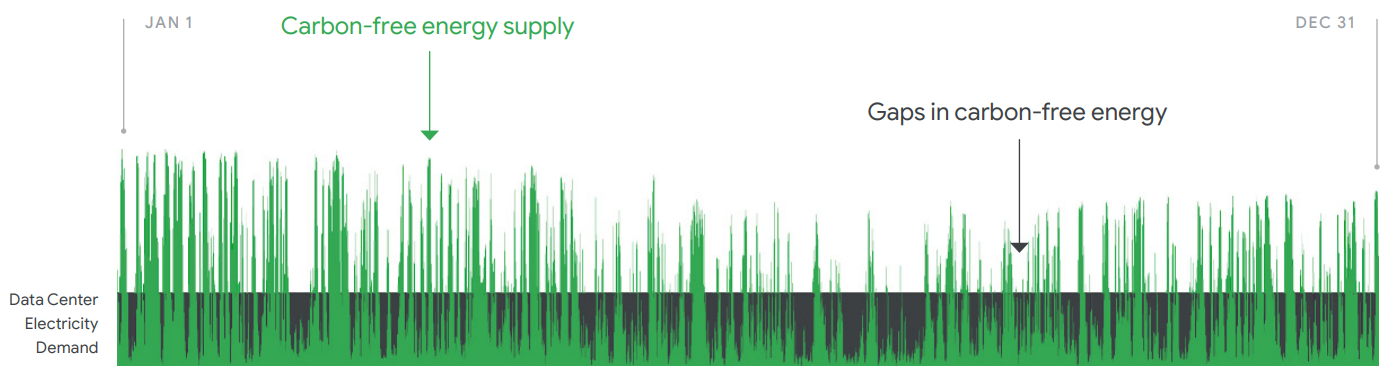
\includegraphics[width=14cm]{images/google-year.png}
  \source{\href{https://www.gstatic.com/gumdrop/sustainability/247-carbon-free-energy.pdf}{source: Google 2021, 24/7 CFE: Methodologies and Metrics}}
           
\end{frame}



\begin{frame}{Introduction}
  
  More generally, 100\% annual matching leads to many challenges 
  from the electricity buyers' and system perspectives: 
  \begin{itemize}
  \item No \alert{simultaneity} - variable generation of wind and solar power is not aligned with the 
  buyers' electricity consumption profile.
  \item Lack of \alert{additionality} - some buyers procure unbundled guarantees of origin from existing 
  facilities, which does not lead to additional renewable generation.
  \item Displaced \alert{location} - some buyers procure PPAs from locations far away 
  from their consumption, where there is no way to transmit the electricity to the demand.
  \item Exposure to \alert{risk} - electricity buyers are exposed to price volatility 
  in local electricity markets, since they still have to procure electricity to cover
  the difference between demand and supply.
  \item Need for \alert{backup} - the rest of the electricity system still has to 
  maintain backup and flexibility options for hours with low renewable generation.
  \end{itemize}
  
\end{frame}



\begin{frame}{24/7 carbon-free energy}

  \centering

  There is growing interest from leaders in voluntary clean
  electricity procurement to cover their consumption 
  with clean energy supply on a \alert{truly 24/7 basis}. \\
  \vspace{0.3cm}
  Achieving 24/7 Carbon-Free Energy (CFE) means that every kilowatt-hour of electricity consumption is met
  with carbon-free electricity sources, \alert{every hour of every day}.
  
\end{frame}



\begin{frame}{Yearly versus hourly matching}
  
  24/7 CFE procurement has potential benefits over the 100\% renewable matching:
  
  \begin{itemize}
  \item Ensure match of electricity consumption with carbon-free resources 
        on an \alert{hourly basis}.
  \item Enable much \alert{deeper reductions in CO$_2$ emissions} associated 
        to buyer's electricity consumption.
  \item Ensure that contracted power is \alert{additional} (i.e. leads to new capacity).
  \item Ensure that power comes from the \alert{same bidding zone}.
  \item Enable technology-neutral procurement of \alert{carbon-free} rather than renewable technologies 
        (such as advanced clean dispatchable power generation and long-duration energy storage).
  \end{itemize}
  
\end{frame}

\begin{frame}{24/7 carbon-free energy}
  
  \begin{columns}[T]
  \begin{column}{8cm}

    \begin{itemize}
    \item The \hrefc{https://www.un.org/en/energy-compacts/page/compact-247-carbon-free-energy}{24/7 Carbon-free Energy Compact} 
    initiative was launched in 2021 by Sustainable Energy for All and the United Nations. 
    It now includes more than 80 companies, policymakers, investors, and organizations 
    on a mission to realize a 24/7 Carbon-Free Energy future. 

    \item One of the front runners in the 24/7 initiative is Google Inc. In 2020 the company committed 
    \hrefc{https://www.gstatic.com/gumdrop/sustainability/247-carbon-free-energy.pdf}{to the goal} 
    of operating entirely on a 24/7-CFE approach at all its data centres and campuses worldwide by 2030. 
    Shortly after, Google published 
    \hrefc{https://www.gstatic.com/gumdrop/sustainability/policy-roadmap-carbon-free-energy.pdf}{a policy roadmap} 
    on achieving the 24/7-CFE goal.

    \end{itemize}
  \end{column}

  \begin{column}{8cm}
    \centering
    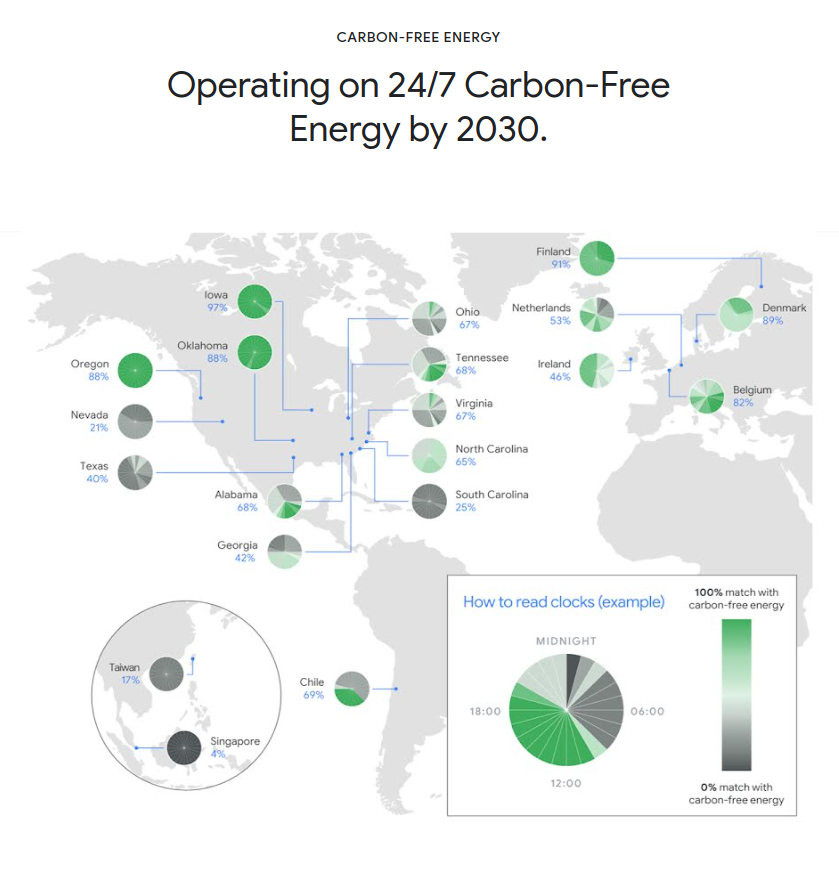
\includegraphics[width=7.5cm]{images/247-google-web.png}
    \vspace{.1cm}
  \end{column}

  \source{\href{https://sustainability.google/progress/energy/}{Google Inc.}}
  \end{columns}
  
\end{frame}



\begin{frame}{Fresh research items}

  Reference to Princeton studies, TU Berlin study 1, IEA report, etc.

\end{frame}


\begin{frame}{Narrow down focus and outline motivation for our new study}

A growing interest from C\&I sector companies to pursue 24/7 CFE \\
A subset of C\&I, like data center operators, have the potential to use spatial and temporal flexibility to achieve high 24/7 CFE easier and help others \\
The first study on space and time load-shifting load management for flexible C\&I that pursue 24/7 carbon-free electricity procurement goals \\

\end{frame}

\begin{frame}{Focus of the study}

  In this study, we focus our analysis on \alert{space-time load-shifting} provided by flexible electricity consumers, such as data centers.
  Thus, in the context of this study, buyers committed to 24/7 CFE procurement can \\
  - shift loads across \alert{time} (via job scheduling); \\
  - shift loads across \alert{space} (via service migration); \\
  - both of the above, i.e., co-optimization of space-time flexibility.

  \vspace{0.3cm}
  We aim to answer the following quesitons:
  \begin{itemize}
    \item To which extent can load-shifting flexibility reduce the \alert{means and costs} of hourly clean energy matching?\\ 
    \item Investigate \alert{individual effects} of space/time flexibility, as well as their \alert{interplay}.\\
    \item How the flexibility value varies across data center \alert{locations} and \alert{years}.\\
    \item ...
  \end{itemize}

\end{frame}


%----------------------------------------
%----------------------------------------

\section{Methodology}


\begin{frame}
  \frametitle{A quick overview}


{\small
  \begin{itemize}
    
    \item The optimization model is based on \hrefc{https://github.com/PyPSA/pypsa-eur}{PyPSA-Eur} -- a widely-used open-source model of the European energy system.

    \item In this study, we build upon the mathematical model of 24/7 clean energy procurement
    developed in the former work of authors: \hrefc{https://zenodo.org/record/7180097}{System-level impacts of 24/7 carbon-free electricity procurement in Europe} (October 2022)
    
    \item We encode a set of new equations and routines, which allow for incorporating spatial (service migration) and temporal (job scheduling) load management systems for data centers.

    \item ... 
    % \item We compare 100\% annual matching with renewable energy versus 
    % different targets for hourly CFE matching.

    % \item We place C\&I consumers committed to a clean energy procurement in a 
    % selection of European countries: Germany, Denmark, Ireland and the Netherlands.
    % These countries differ in patterns of electricity demand, renewable potentials,
    % national energy and climate policies, legacy fleets of generation capacities, degree 
    % of interconnectons, etc. Apart form that, we consider different C\&I participation rates, a wide palette 
    % of CFE generation technologies available for 24/7 consumers, 
    % and two years (2025 and 2030). These differences help to understand and generalize 
    % the impacts of 24/7 CFE procurement.
    
  \end{itemize}
}

\end{frame}


\begin{frame}
  \frametitle{PyPSA project}

\begin{columns}[T]
\begin{column}{7cm}

{\small
  \begin{itemize}
  \item \hrefc{https://pypsa.org/}{pypsa.org} project provides a free, user-friendly and performant model environment to support a smooth energy transition around the world. 
  \item The project includes individual packages that enable to go all the way from data processing (e.g., calculating renewable energy potentials or collecting energy assets data) to creating complex energy optimization problems. All packages are build in a modular sense so that they may be used independently from each other but interact easily.
  \item PyPSA development and maintenance is coordinated by the Department of Energy Systems @ TU~Berlin \hrefc{https://www.tu.berlin/en/ensys/about-us}{(ENSYS)}.  
  \end{itemize}
}
\end{column}
\begin{column}{9cm}

\centering
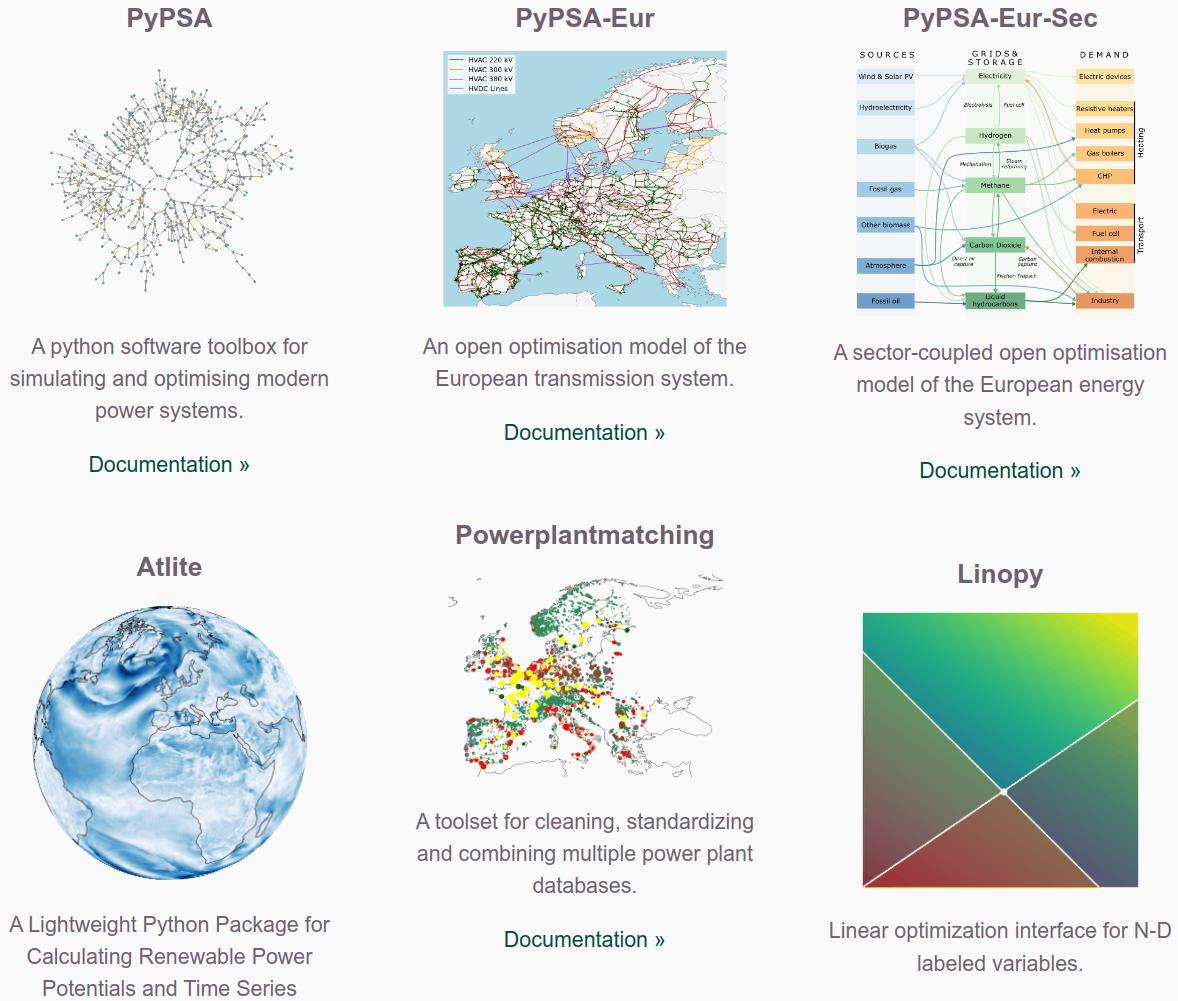
\includegraphics[width=8.5cm]{images/pypsa-web.png}
\source{\href{https://pypsa.org/}{pypsa.org}}

\end{column}
\end{columns}

\end{frame}


% \item PyPSA is used worldwide by dozens of research institutes and companies.\\
% See \hrefc{https://pypsa.readthedocs.io/en/latest/users.html}{list of users}.


\begin{frame}
  \frametitle{PyPSA-Eur: open models of the European energy system}

  \begin{columns}[T]
  \begin{column}{7cm}
  {\small
  \begin{itemize}
  \item PyPSA-Eur is an open model of the European power system at the transmission network 
  level that covers the full ENTSO-E area.
  \item Only freely available and open data.
  \item Automated and configurable software pipeline from raw data to optimised electricity system.
  \item Adjustable temporal and spatial resolution.
  \item See \hrefc{https://pypsa-eur.readthedocs.io/en/latest/}{documentation}
  and \hrefc{https://docs.google.com/presentation/d/1mzj4X9uuO58gUvkhVMRCFWOJUWbs6NR9SNZe-RIkkNo/edit?usp=sharing}{feature summary} 
  for more details.
  \item PyPSA-Eur{\bf-Sec} version of the model adds building heating, transport and industry sectors, as well as gas networks.
  \end{itemize}
  }
  \end{column}

  \begin{column}{9cm}
    \centering
  {\footnotesize
    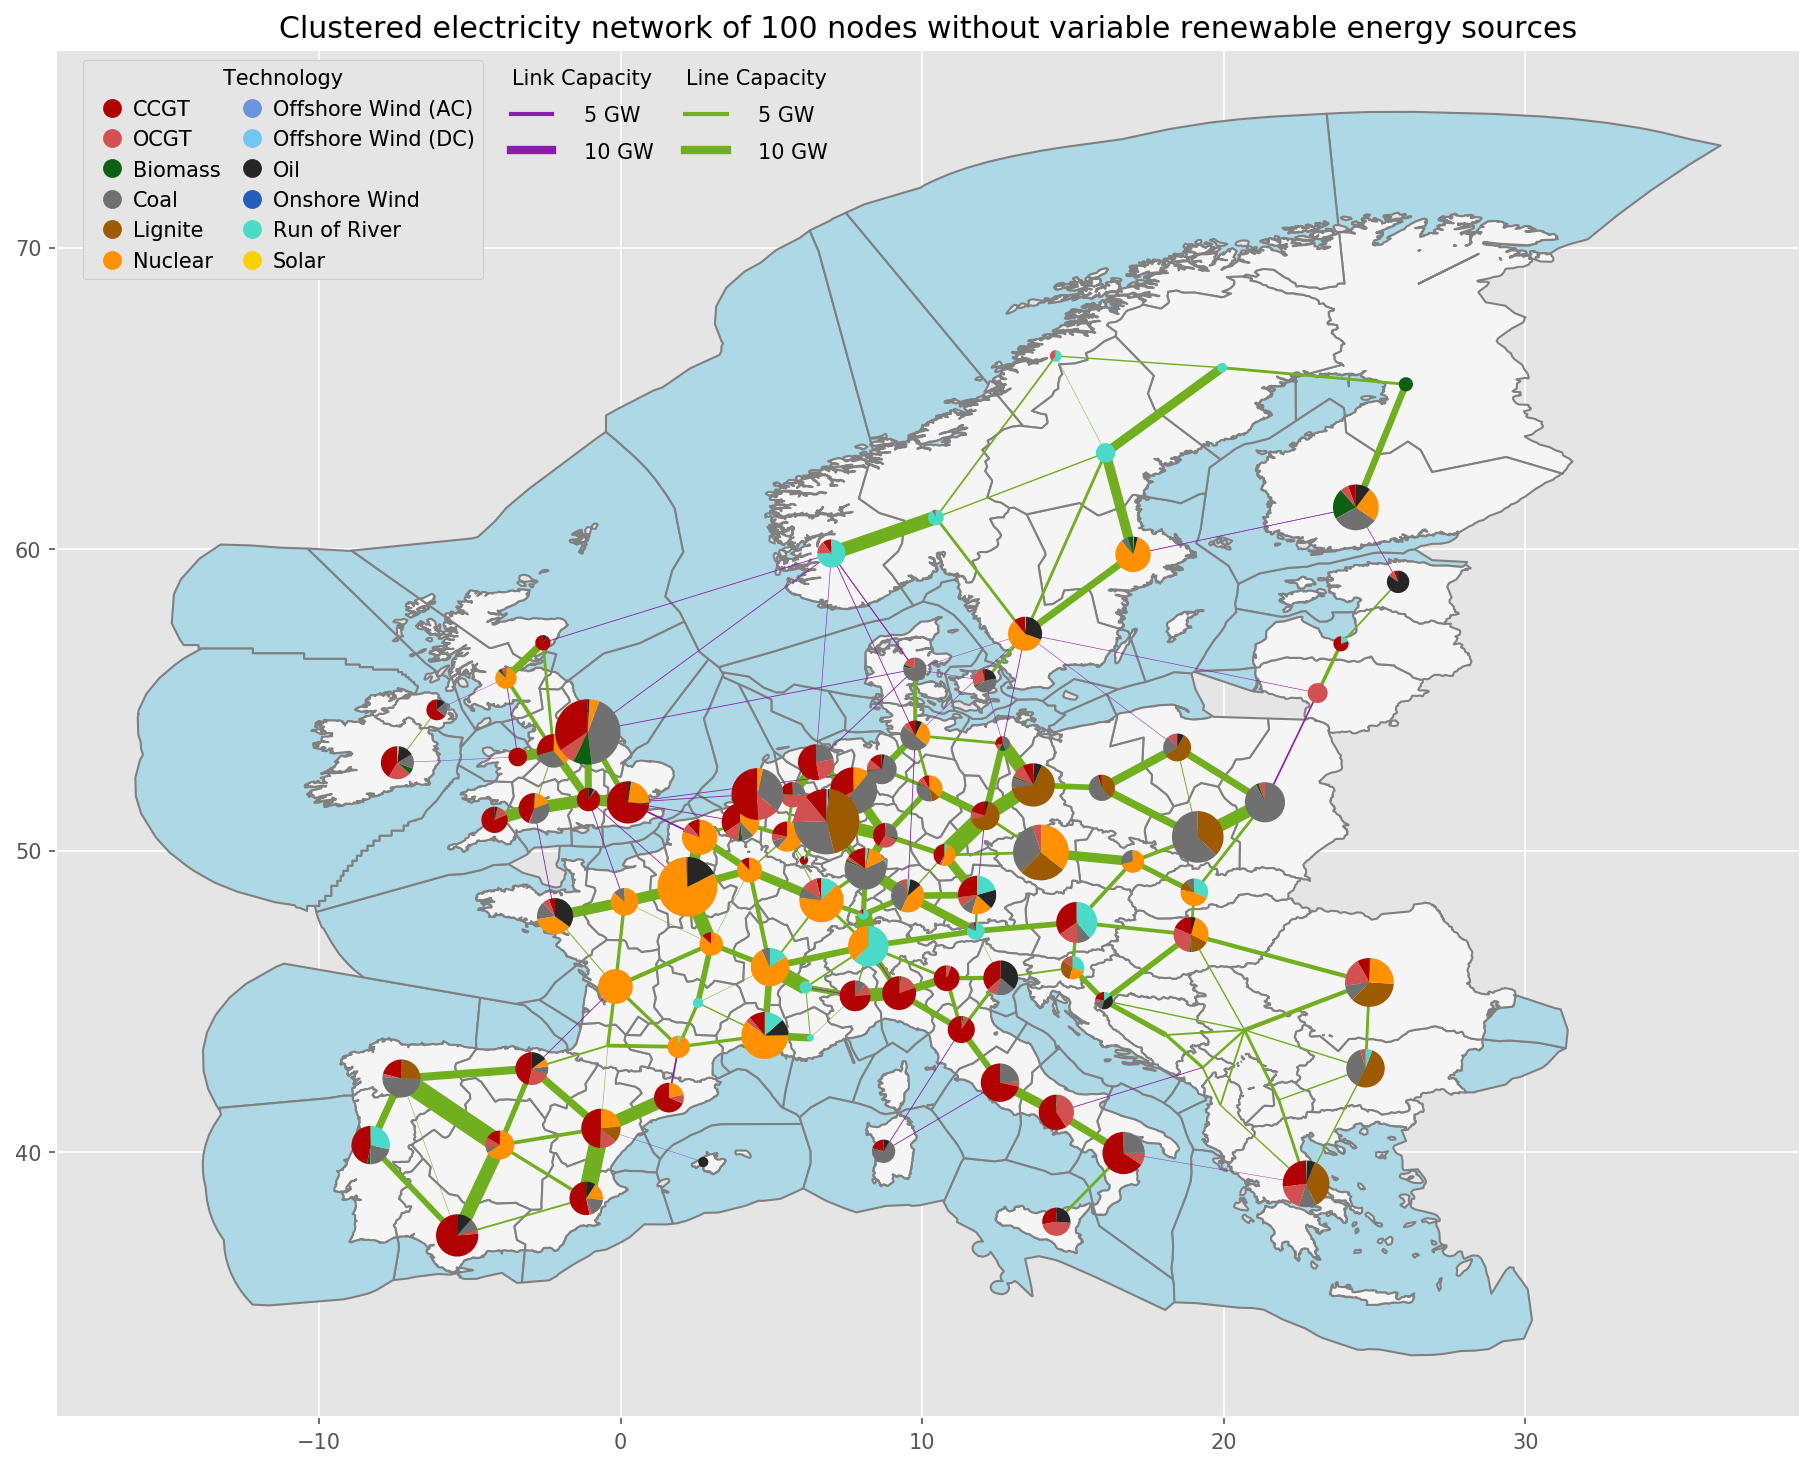
\includegraphics[width=8cm]{images/elec_s_100.png}
  
   \vspace{0.1cm}
   PyPSA-Eur(-Sec) suite of models are available on \hrefc{https://github.com/PyPSA}{GitHub}
  }
  \end{column}
  
  \end{columns}

\end{frame}



\begin{frame}{Modeling 24/7 CFE procurement}
  \begin{columns}[T]
  \begin{column}{7cm}
  {\small

  \begin{itemize}
  \item We implement a set of additional constraints to the PyPSA-Eur 
  to model a situation when a fraction of corporate and industry (C\&I) demand 
  commits to the 24/7~CFE procurement.
  \item The model optimises investment and operational decisions to meet projected
  electricity demand for the 24/7~CFE consumers, as well as
  the demand of other consumers in the European electricity system, while meeting all
  relevant engineering, reliability, and policy constraints.
  \end{itemize}
  }
  \end{column}

  \begin{column}{9cm}
  \centering
  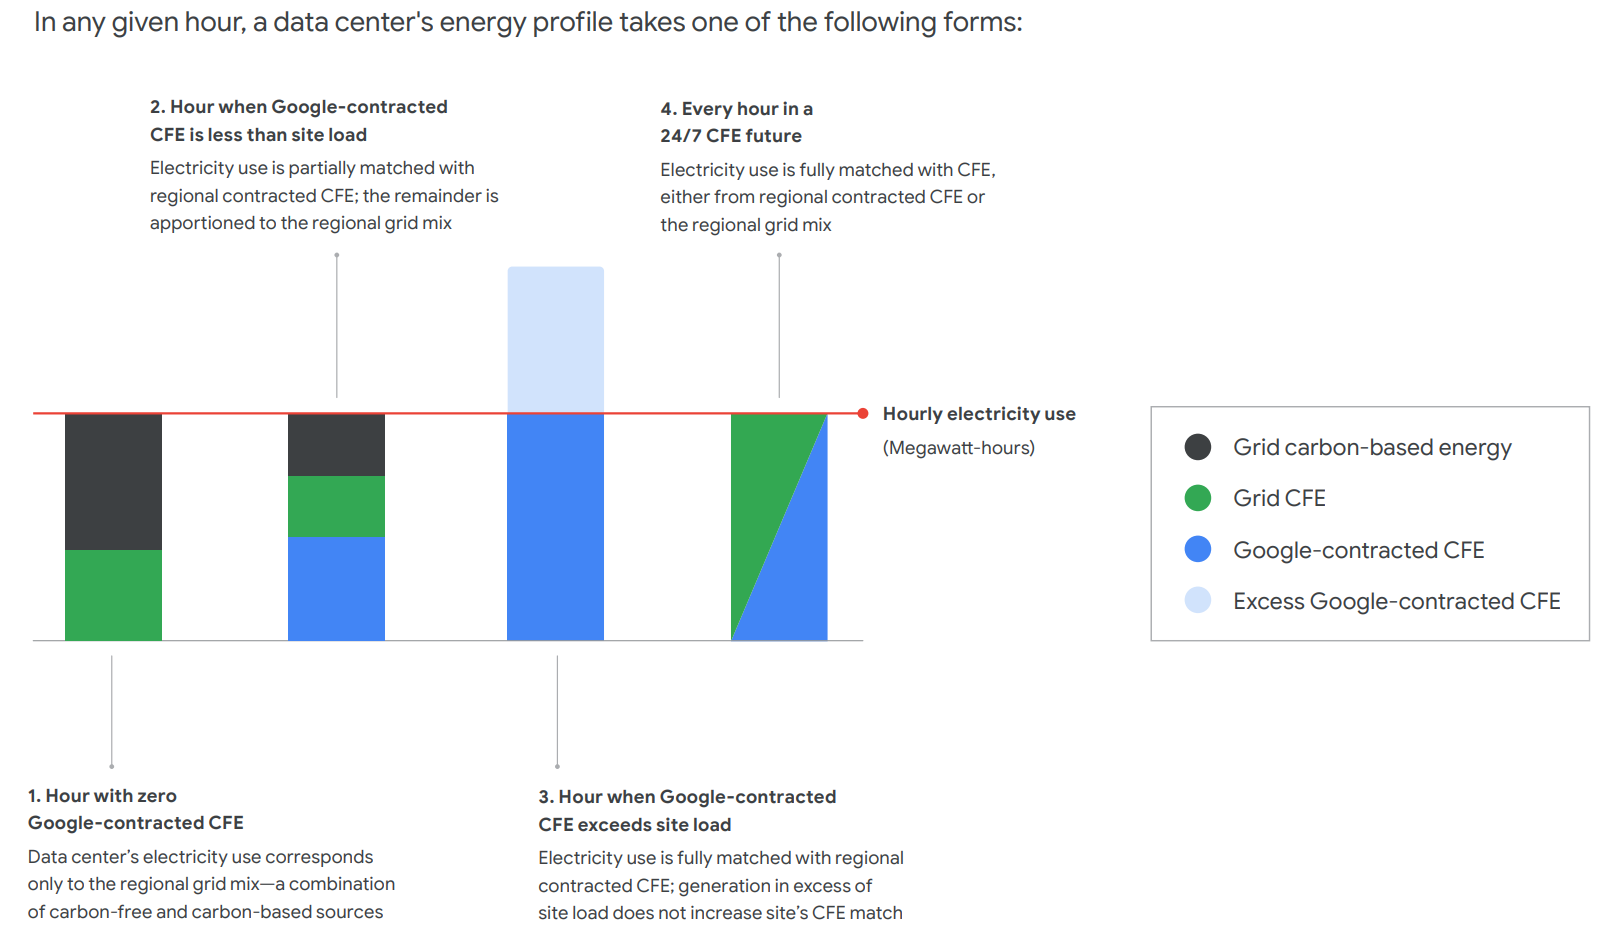
\includegraphics[width=8.5cm]{images/247-concept.png}
  {\footnotesize
  The methods are based on the Google's CFE procurement framework, presented in paper
  \hrefc{https://www.gstatic.com/gumdrop/sustainability/24x7-carbon-free-energy-methodologies-metrics.pdf}{"24/7 Carbon-Free Energy: Methodologies and Metrics"}
  }
  \source{\href{https://www.gstatic.com/gumdrop/sustainability/24x7-carbon-free-energy-methodologies-metrics.pdf}{source: Google 2021, 24/7 CFE: Methodologies and Metrics}}
  \end{column}

  \end{columns}

\end{frame}



\begin{frame}{Implementation of C\&I demand and supply}

  {\small

  The model optimizes a portfolio of carbon-free generation and storage technologies 
  procured by the participating C\&I consumers. The portfolio assets have to be located 
  in the same market zone.

  The hourly demand of C\&I consumers $d_t$ for hour $t$ can be met 
  by a combination of the following: \\
    \begin{itemize}
      \item dispatch $g_{r,t}$ of procured CFE generators $r\in CFE$ 
      \item dispatch $\bar{g}_{s,t}$ of procured storage technologies $s\in STO$
            (requires charge $\ubar{g}_{s,t}$)
      \item imports from the grid $im_t$.
    \end{itemize}
    }

\begin{columns}

  \begin{column}{7cm}
  \begin{equation*}
  \sum_{r\in CFE} g_{r,t} + \sum_{s\in STO} \left(\bar{g}_{s,t} - \ubar{g}_{s,t}\right) - ex_t + im_t  =  d_t \hspace{.7cm} \forall t
  \end{equation*}

  \vspace{0.3cm}
  {\small NB: the excess from the local supply $ex_t$ can either be sold to the grid 
  at market prices or curtailed.}
  \end{column}

\begin{column}{5cm}
\centering
\begin{circuitikz}
  \draw (0,13.5) to [short,i^=$im_t$]  (1.5,13.5) to (1.5,13);
  \draw [ultra thick] (0,13) node[anchor=south]{} -- (4,13);
  \draw(2.5,13) |- +(0,0.5) to [short,i^=$ex_t$] +(1.5,0.5);
  \draw (0.5,13) -- +(0,-0.5) node[sground]{};
  \draw (2,12) node[vsourcesinshape, rotate=270](V2){}
  (V2.left) -- +(0,0.6);
  \draw (3.5,13) -- (3.5,12.4);
  \draw (3.5,12.4) to [esource] (3.5,11.7);
  \draw (0.5,11) node{$d_t$};
  \draw (2,11) node{$g_{CFE,t}$};
  \draw (3.5,11) node{$g_{STO,t}$};
\end{circuitikz}
\end{column}

\end{columns}

\end{frame}



\begin{frame}{Implementation of 100\% annual matching}

  {\small
  
The \alert{100\% annual matching} is modelled with a constraint (\ref{eqn:RES100}), which requires C\&I consumers 
to purchase enough renewable electricity from the local bidding zone to match all of their electricity consumption
on an annual basis.

\vspace{0.3cm}
More formally, the sum of all dispatch $g_{r,t}$ for RES generators $r\in RES$ over the year $t\in T$ 
is equal to the annual demand $d_t$ of C\&I consumers:
  \begin{equation}
    \sum_{r\in RES, t\in T} g_{r,t} = \sum_{t\in T} d_t
  \label{eqn:RES100}
  \end{equation}
  }
\end{frame}


\begin{frame}{Implementation of 24/7 CFE matching}

  {\small

  The \alert{24/7 CFE matching} is modelled with a constraint (\ref{eqn:CFE}), 
  which matches demand of C\&I consumers with carbon-free resources on an hourly basis. 

  More formally, the constraint states that sum over generators from procured CFE resources $r\in CFE$,
  discharge and charge from storage technologies $s\in STO$,
  as well as import from the grid $im_t$ multiplied by the grid's CFE factor $CFE_t$
  must be higher or equal than a certain CFE target $x$ multiplied with the total load:
  \vspace{0.1cm}
  \begin{equation}
  \sum_{r\in CFE, t\in T} g_{r,t} + \sum_{s\in STO, t\in T} \left(\bar{g}_{s,t} - \ubar{g}_{s,t}\right) - \sum_{t\in T} ex_t + \sum_{t\in T} CFE_t \cdot im_t \geq x \cdot \sum_{t\in T} d_t
  \label{eqn:CFE}
  \end{equation}
  \vspace{0.1cm}
  \noindent\fbox{%
    \parbox{\textwidth}{%
  The \alert{CFE Score} $x$~[\%] measures the degree to which hourly electricity consumption 
  is matched with carbon-free electricity generation within the regional grid.
  }}

  \noindent\fbox{%
    \parbox{\textwidth}{%
  Note that the grid CFE factor $CFE_t$ is affected by capacity procured by C\&I consumers. This
  introduces a nonconvex term to the optimization problem. The nonconvexity can be avoided by treating 
  the grid CFE factor as a parameter that is iteratively updated (starting with $CFE_t =0 \,~\forall t$). 
  Similarly to the \hrefc{https://acee.princeton.edu/24-7/}{Xu et al. (2021)} study, 
  we find that one forward pass (i.e. 2 iterations) yields very good convergence.
  }}
  }

\end{frame}



\begin{frame}{Implementation of 24/7 CFE matching}

  {\small

  The excess generation $ex_t$ from the procured resources represents clean electricity sold to the rest of the grid. 
  The \alert{excess is not counted toward the CFE score} -- 
  and thus it is subtracted on the left-hand side of the eq. (\ref{eqn:CFE}).

  CFE generation above the demand can be stored and shifted to another hour where procured resources 
  generate less than the C\&I demand, sold to the regional grid as excess $ex_t$
  at {\bf market prices}, or curtailed. 
  The total amount of excess generation is constrained to a certain level on an annual basis. 
  In this study, the limit is set to 20\% of annual 24/7 participating customer's demand:
  \vspace{0.1cm}
  \begin{equation}
  \sum_{t\in T} ex_t \leq ExLimit \cdot \sum_{t\in T} d_t
  \label{eqn:excess}
  \end{equation}

  \noindent\fbox{%
  \parbox{\textwidth}{%
  The constraint (\ref{eqn:excess}) gives the C\&I consumers the flexibility to sell 
  electricity to the regional grid, while avoiding the situation that sales to the grid 
  become significantly larger than supply to the C\&I's own demand.
  }}

  \noindent\fbox{%
  \parbox{\textwidth}{%
  The {\bf market prices} are derived from the dual variable of each zone's
  energy balance constraint. An infinitely small relaxation of the 
  constraint, i.e., one unit of load less to be met, returns the 
  marginal costs of providing that unit, which can be used as the
  electricity price indicator in a competitive market.
  }}
  }

\end{frame}



\begin{frame}{CFE factor of the regional grid}

  {\small

  The \alert{grid CFE factor} $CFE_t$ in eq. (\ref{eqn:CFE}) defines the share of 
  carbon-free electricity  in grid imports by C\&I consumers following 24/7 approach. 
  The factor depends on the generation mix in the region where C\&I consumers are located, 
  as well as on the generation mix in other regions from which electricity is imported
  to the local region ($import_t$). 

  \begin{columns}
    \begin{column}{8cm}

  Using the notation on the right, the average cleanness 
  of the rest of the electricity system is:
  \begin{equation*}
  ImportCFE_t = \frac{A_t}{A_t + D_t}
  \end{equation*}

  The CFE factor of grid supply\footnote{Note 
  that generators contracted by 24/7 consumers (C) are excluded from the grid supply.} 
  for a given hour $t$ is:
  
  \begin{equation*}
  CFE_t = \frac{B_t + ImportCFE_t * import_t}{B_t + E_t + import_t}
  \end{equation*}    

  \end{column}

  \begin{column}{5cm}
  \centering
  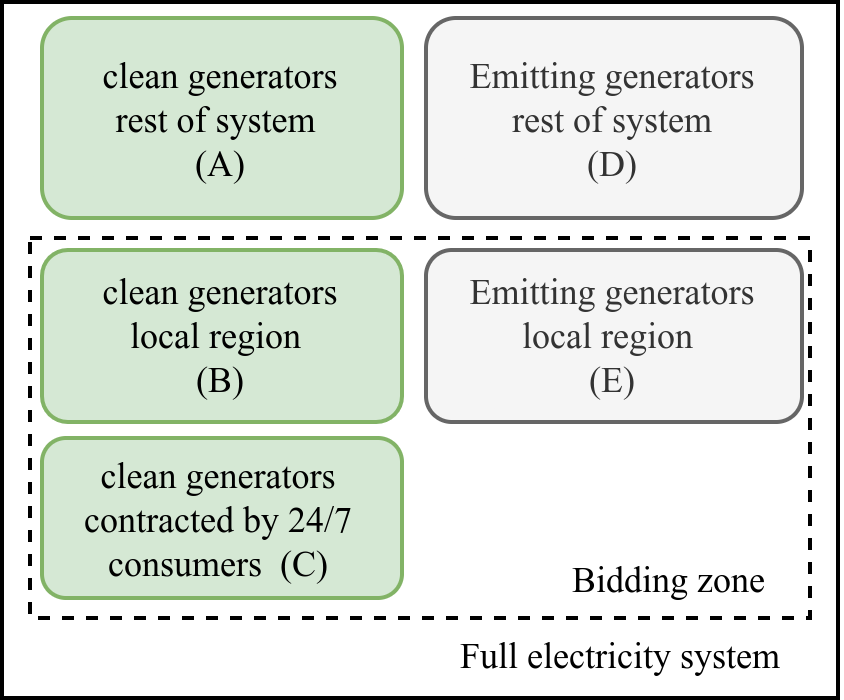
\includegraphics[width=5cm]{images/cfe.png}
  {\scriptsize
  This approach is based on \hrefc{https://acee.princeton.edu/24-7/}{Xu et al. (2021)}
  }
  \end{column}
    
  \end{columns}

  \noindent\fbox{%
  \parbox{\textwidth}{%
  $CFE_t$ can be seen as the percentage of clean electricity in each MWh of imported 
  electricity from the grid to supply participating 24/7 loads in a given hour.
  }}
  }

\end{frame}


\begin{frame}{CO$_2$ emissions rate of the regional grid and 24/7 portfolio, 1/2}

  {\small

  \alert{CO$_2$ emissions} associated with the dispatch of emitting power plants 
  in the European electricity system are part of the model solution.
  We can use this information to calculate (i) the \emph{emissionality} of generation 
  that serves participating 24/7 demand, and (ii) the \emph{avoided emissions}, i.e.,
  the difference in regional CO$_2$ emissions with and without 24/7 procurement. 
  Similarly to the logic of computing the grid CFE factor, 
  we need to consider imported emissions also in this calculation.
  
  First, let $X(D)_t$ be hourly emissions $[tCO_2]$ in the rest of the electricity system. 
  The average emissions rate of the rest of the system is calculated as:

  \begin{equation*}
  SystemEmisRate = \frac{X(D)_t}{A_t + D_t}
  \end{equation*}

  Second, let $Y(E)_t$ be hourly emissions in the regional grid where 24/7 consumers are located.
  The emissions rate of grid supply is then:

  \begin{equation*}
  GridSupplyEmisRate = \frac{Y(E)_t + SystemEmisRate * import_t}{B_t + E_t + import_t}
  \end{equation*}

  }
\end{frame}



\begin{frame}{CO$_2$ emissions rate of the regional grid and 24/7 portfolio, 2/2}

  {\small
  Third, we calculate {CO$_2$ emissions} associated with the electricity consumption of 
  24/7 participating consumers on an hourly basis:
  
  \begin{equation*}
  Emissions_t = GridSupply_t * GridSupplyEmisRate_t
  \end{equation*}

  Now, we have the necessary components to calculate two metrics of interest for our analysis. 
  A first metric is the \alert{average emissions rate of 24/7 consumers}:

  \begin{equation*}
    (C\&I)EmisRate = \frac{\sum_{t\in T} Emissions_t}{\sum_{t\in T} Load_t}
  \end{equation*}

  A second metric is the \alert{avoided emissions} by 24/7 procurement. The calculation is based on the 
  difference between the total {CO$_2$ emissions} in the regional grid where 24/7 consumers are located
  with and without 24/7 procurement (\emph{'247-cfe'} and \emph{'reference'} labels, accordingly):

  \begin{equation*}
    AvoidedEmissions = \sum_{t\in T} Y(E)_t^{reference} - \sum_{t\in T} Y(E)_t^{247-cfe}
  \end{equation*}
  }

\end{frame}




\begin{frame}{Spatial load shifting problem}

  \centering
  \includegraphics[height=8.3cm]{images/space-flex.pdf}
  
\end{frame}

\begin{frame}{Temporal load shifting problem}

  \centering
  \includegraphics[height=8.1cm]{images/time-flex.pdf}
  
\end{frame}


\begin{frame}{Data center parametrization}

  \begin{columns}[T]
  \begin{column}{5cm}

  \centering
  \vspace{0.3cm}
  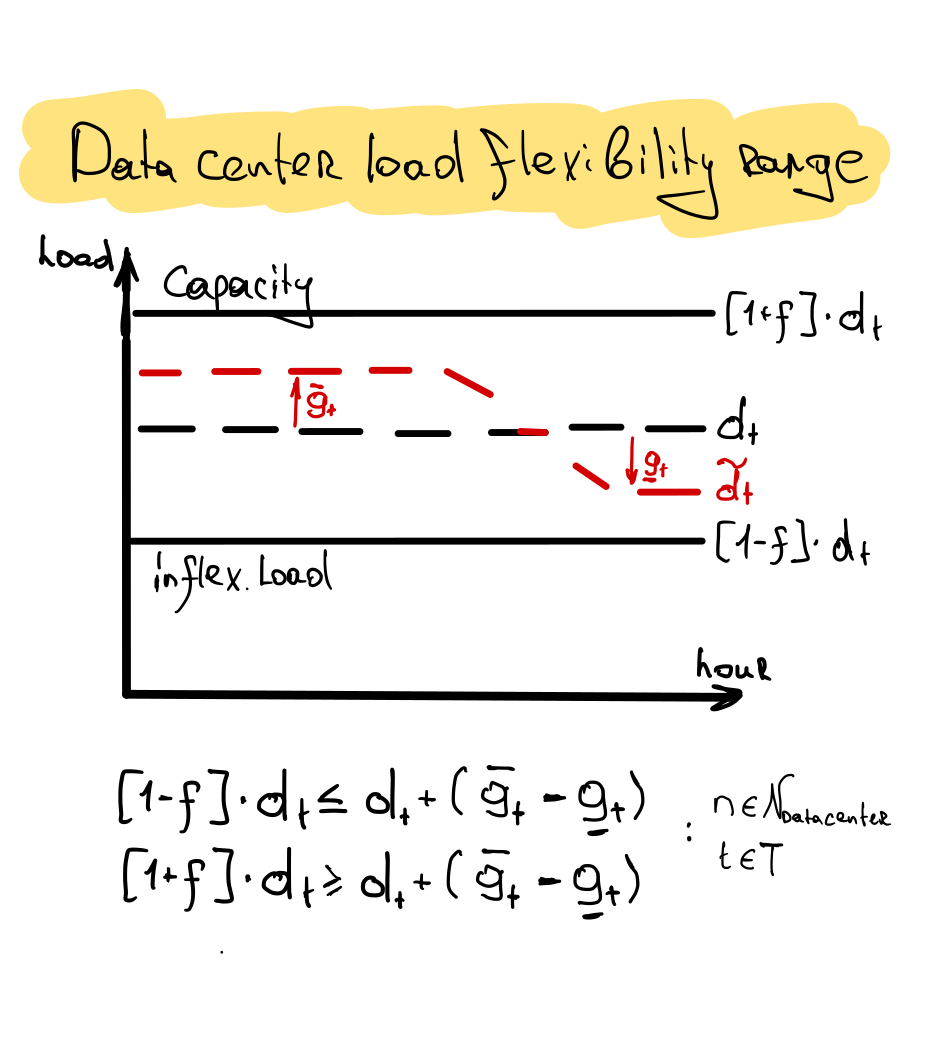
\includegraphics[width=5cm]{images/load_flex.png}

  \vspace{0.1cm}
  {\scriptsize
   
  }
  \end{column}

  \begin{column}{10cm}
  {\small
  \begin{itemize}

  \item \alert{Multiple data centers} (consumers following 24/7 approach) can be located 
        in any bidding zone of the ENTSO-E area

  \item Data centers a have a nominal load of \alert{100~MW} (baseload profile)

  \item Requested load $\widetilde{d}_t$ at any data center can deviate from the nominal load $d_t$. 
        Requested load is constrained by the \alert{data center capacity} 
        (an upper limit) and the \alert{inflexible loads} (a lower limit)
  
  \item Data centers can \alert{shift loads across space} (service migration)
  
  \item Data centers can \alert{shift loads across time} (via job scheduling)

  \item Adjusted scenario palette and new metrics to focus on flexibility \& 24/7 CFE procurement
  
  \end{itemize}
  }

  \end{column}
  \end{columns}

\end{frame}


%----------------------------------------
%----------------------------------------
\section{Study design}

\begin{frame}{EU-wide network simulation}

  \begin{columns}[T]
  \begin{column}{10cm}

  \centering
  \includegraphics[width=10cm]{../results/report-EU-1H-GoogleDC-allflex/map.pdf}

  {\scriptsize
  NB power generation capacity fleet before optimization stage\\
  }

  \end{column}

  \begin{column}{6cm}
  {\small
  \begin{itemize}
  \vspace{-.1cm}
  \item European power system (ENTSO-E area) clustered to \alert{37 zones}.
  \item Each zone represents an individual country. Some countries
  that straddle different synchronous areas are split to individual
  bidding zones, such as DK1 (West) and DK2 (East).
  \item \alert{Co-optimization} of investment and power dispatch
  decisions to meet electricity demand of datacenters (24/7 CFE consumers), as well as the demand of other
  consumers in the European electricity system. 
  \item \alert{Hourly resolution} (no time sampling).
  
  \end{itemize}
  }

  \end{column}
  \end{columns}

\end{frame}


\begin{frame}{Datacenters: Google DC locations}

  \begin{columns}[T]
  \begin{column}{10cm}

  \centering
  \includegraphics[width=9cm]{../results/report-EU-1H-GoogleDC-allflex/map-DC.pdf}


  \end{column}

  \begin{column}{6cm}
  {\small
  \begin{itemize}

  \item Data centers are located in \\ \alert{IE, DK1, FI, BE, NL}
  \item Nominal load is 100~MW (baseload)
  \item Flexibility scenarios: \\
        1. Shifting loads via virtual links \\ 
        2. Shifting loads in time \\ 
        3. Both mechanisms
  \item Flexibility range: $f \in \{0,0.05,0.1,0.2,0.4\}$ 
  \item Scenario year: 2025
  \item 24/7 CFE targets: 100\% and 90\%
  \item Technology palettes with/wo LDES
  
\end{itemize}
  }

  \end{column}
  \end{columns}

\end{frame}



\begin{frame}{Scenario setup 1/3}
 
  \begin{columns}[T]
  \begin{column}{7.2cm}

  \centering
  \vspace{0.3cm}
  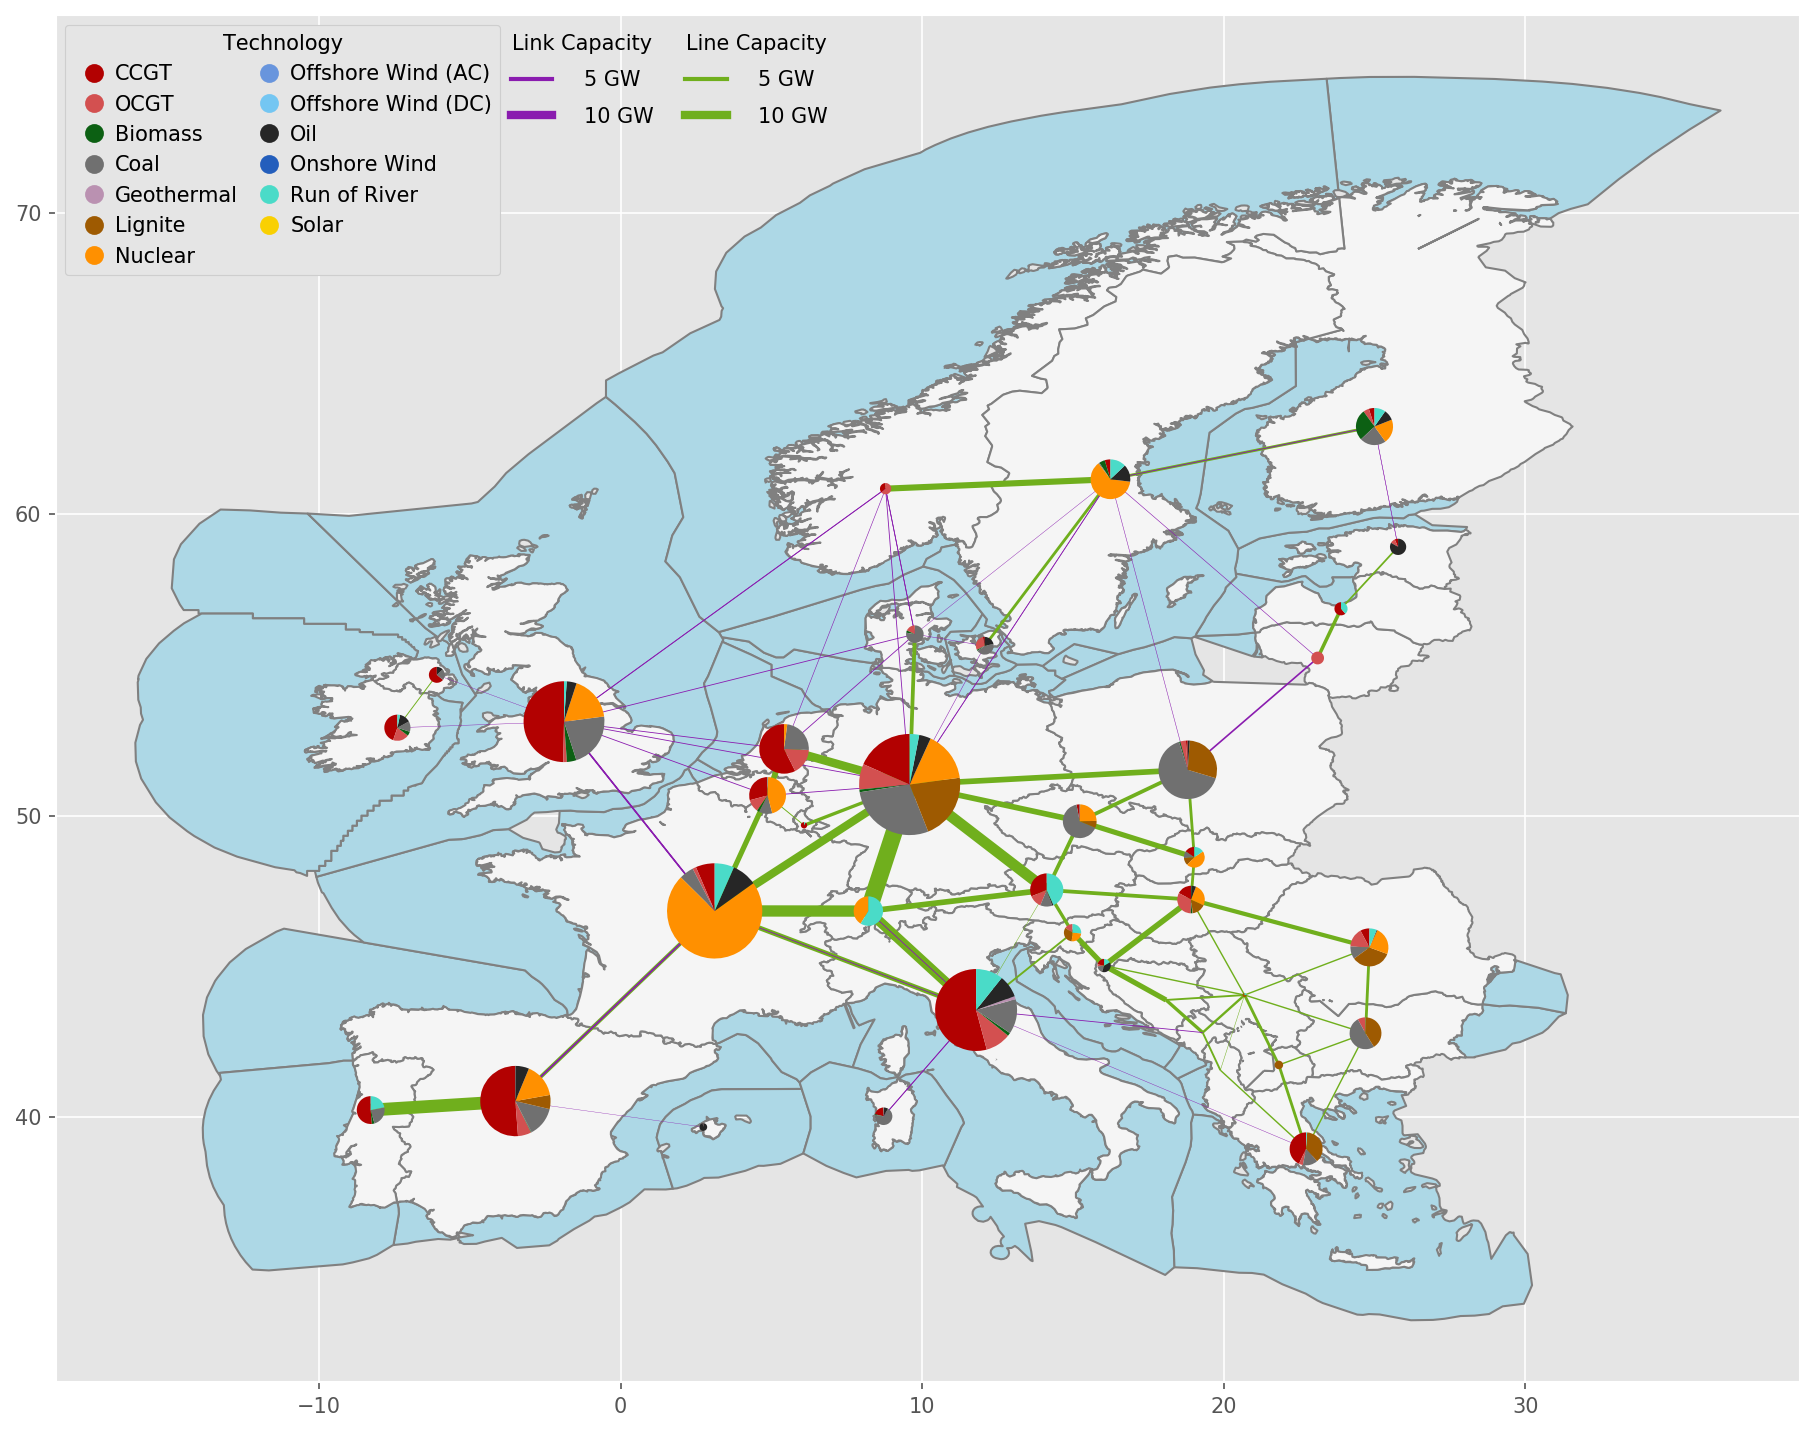
\includegraphics[width=7.5cm]{images/elec_s_37.png}

  {\footnotesize 
  PyPSA-Eur network clustered to 37 zones
  }
  \end{column}

  \begin{column}{8.5cm}
  {\footnotesize 
  \begin{itemize}
  \item In each scenario, we model the full European power system 
  clustered to \alert{37 zones}. 
    
  \item Each zone represents an individual country. Some countries
  that straddle different synchronous areas are split to individual bidding zones, 
  such as DK1 (West) and DK2 (East).

  \item Consumers following 24/7 approach can be located in one of the \alert{four zones}: 
  Ireland, Denmark (zone DK1), Germany and the Netherlands.
    
  \item We assume that all consumers committed to 24/7 matching, form an alliance and sign contracts 
  with CFE generators so that their aggregated consumption can be matched 
  on an hour-by-hour basis with clean generation to achieve a given CFE matching score.\footnote
 {{\scriptsize In reality, C\&I participants can also pursue hourly matching strategies
  independently based on their own specific load profiles. 
  See \hrefc{https://zenodo.org/record/7082212}{Qingyu \& Jenkins (2022)} study investigating this case.}}
  
  \end{itemize}
  }
  
  \end{column}
  \end{columns}

\end{frame}



\begin{frame}{Scenario setup 2/3}

  {\footnotesize 

  We assume that 24/7 consumers have an access to a wide palette
  of carbon-free technologies\footnote{{\scriptsize We consider carbon-free power generation
  technologies that we believe can play important roles in facilitating CFE matching on hourly basis, 
  while enabling deeper decarbonization of electricity systems at the same time. Technology inclusivity is a 
  \hrefc{https://www.gstatic.com/gumdrop/sustainability/24x7-carbon-free-energy-methodologies-metrics.pdf}{principle} 
  of the 24/7 CFE methodology.}} that are either available on the European market now
  or expected to be available for a commercial scale up in the near future. 
  We formulate three scenarios grouping generators by a degree of technological
  maturity as of now:

  \centering
  \begin{table}[h]
  \begin{tabular}{ccc}
    \hline
    \alert{Palette 1} & \alert{Palette 2} &  \alert{Palette 3} \\
    \hline
      onshore wind & onshore wind  & onshore wind \\ 
    \hline
      utility scale solar & utility scale solar  & utility scale solar \\
    \hline
      battery storage & battery storage  & battery storage \\
    \hline
      - & LDES\footnote{{\scriptsize Long-duration energy storage (LDES).}} & LDES \\
    \hline
      - & - & Allam cycle with CCS\footnote{{\scriptsize Allam cycle is a natural gas power plant 
      with up to 100\% of carbon capture and sequestration.}}  \\
    \hline
      - & - & Advanced dispatchable generator\footnote{{\scriptsize A stand-in for clean dispatchable technologies, 
      such as advanced geothermal (closed-loop) or nuclear systems. See e.g., \hrefc{https://www.eavor.com/}{Eavor} 
      developing a promising solution for clean baseload \& dispatchable power with a potential
      for a commercial scale up in Europe.}} \\  
  \end{tabular}
  \end{table}
  }
  \vspace{0.5cm}

\end{frame}



\begin{frame}{Scenario setup 3/3}

  {\footnotesize 
  \begin{itemize}

  \item We model various procurement policies and targets. The scenarios include: \\
  (i) \alert{24/7 CFE matching} with seven different CFE scores in a range from 80\% to 100\%, \\
  (ii) \alert{100\% annual renewable matching} -- the best case scenario for the annual matching policy, \\
  (iii) \alert{A reference case} when 24/7 consumers cover their load purely with grid purchases 
  without any policy regarding the origin of electricity.

  \item We focus on two periods: \alert{2025} and \alert{2030}. The two periods differ by \\ 
  (i) Technology cost assumptions, \\
  (ii) National renewable expansion pathways,\\
  (iii) Power plant fleet (changes take place due to decommissioning based on generators' 
  age or national policies), \\
  (iv) System-wide assumptions, such as price for EU ETS allowances.

  \item We conduct an analysis for different rates of participation. The two scenarios 
  assume that \alert{10\%} and \alert{25\%} of commercial and industrial load
  in a given zone participate in 24/7 CFE matching.

  \item Finally, we conduct an analysis for different (synthetic) load profiles of C\&I participants, which
  represent a \alert{'baseload'} (flat), a \alert{'datacenter'}, and an \alert{'industry consumer'} consumption patterns.   

  \end{itemize}
  }
\end{frame}


\begin{frame}{Technology palettes span different commercial maturities}

  {\small

  We consider carbon-free technologies available today and that could scale up soon.
  We formulate \alert{three palettes} grouping generators by a degree of technological
  maturity:

  \centering
  \begin{table}[h]
  \begin{tabular}{ccc}
    \hline
    \alert{Palette 1} & \alert{Palette 2} &  \alert{Palette 3} \\
    \hline
      onshore wind & onshore wind  & onshore wind \\
    \hline
      utility scale solar & utility scale solar  & utility scale solar \\
    \hline
      battery storage & battery storage  & battery storage \\
    \hline
      - & LDES\footnote{{\scriptsize Long-duration energy storage (LDES).}} & LDES \\
    \hline
      - & - & Allam cycle with CCS\footnote{{\scriptsize Allam cycle is a natural gas power plant
      with up to 100\% of carbon capture and sequestration.}}  \\
    \hline
      - & - & Advanced dispatchable generator\footnote{{\scriptsize A stand-in for clean dispatchable technologies,
      such as advanced geothermal (closed-loop) or nuclear systems.}} \\
  \end{tabular}
  \end{table}
  }
  \vspace{0.5cm}

\end{frame}


%----------------------------------------
%----------------------------------------
\section{Data sources}


\begin{frame}{Summary of data sources: electricity grid}
 
  \begin{columns}[T]
  \begin{column}{7cm}

  \vspace{0.3cm}
  \centering

  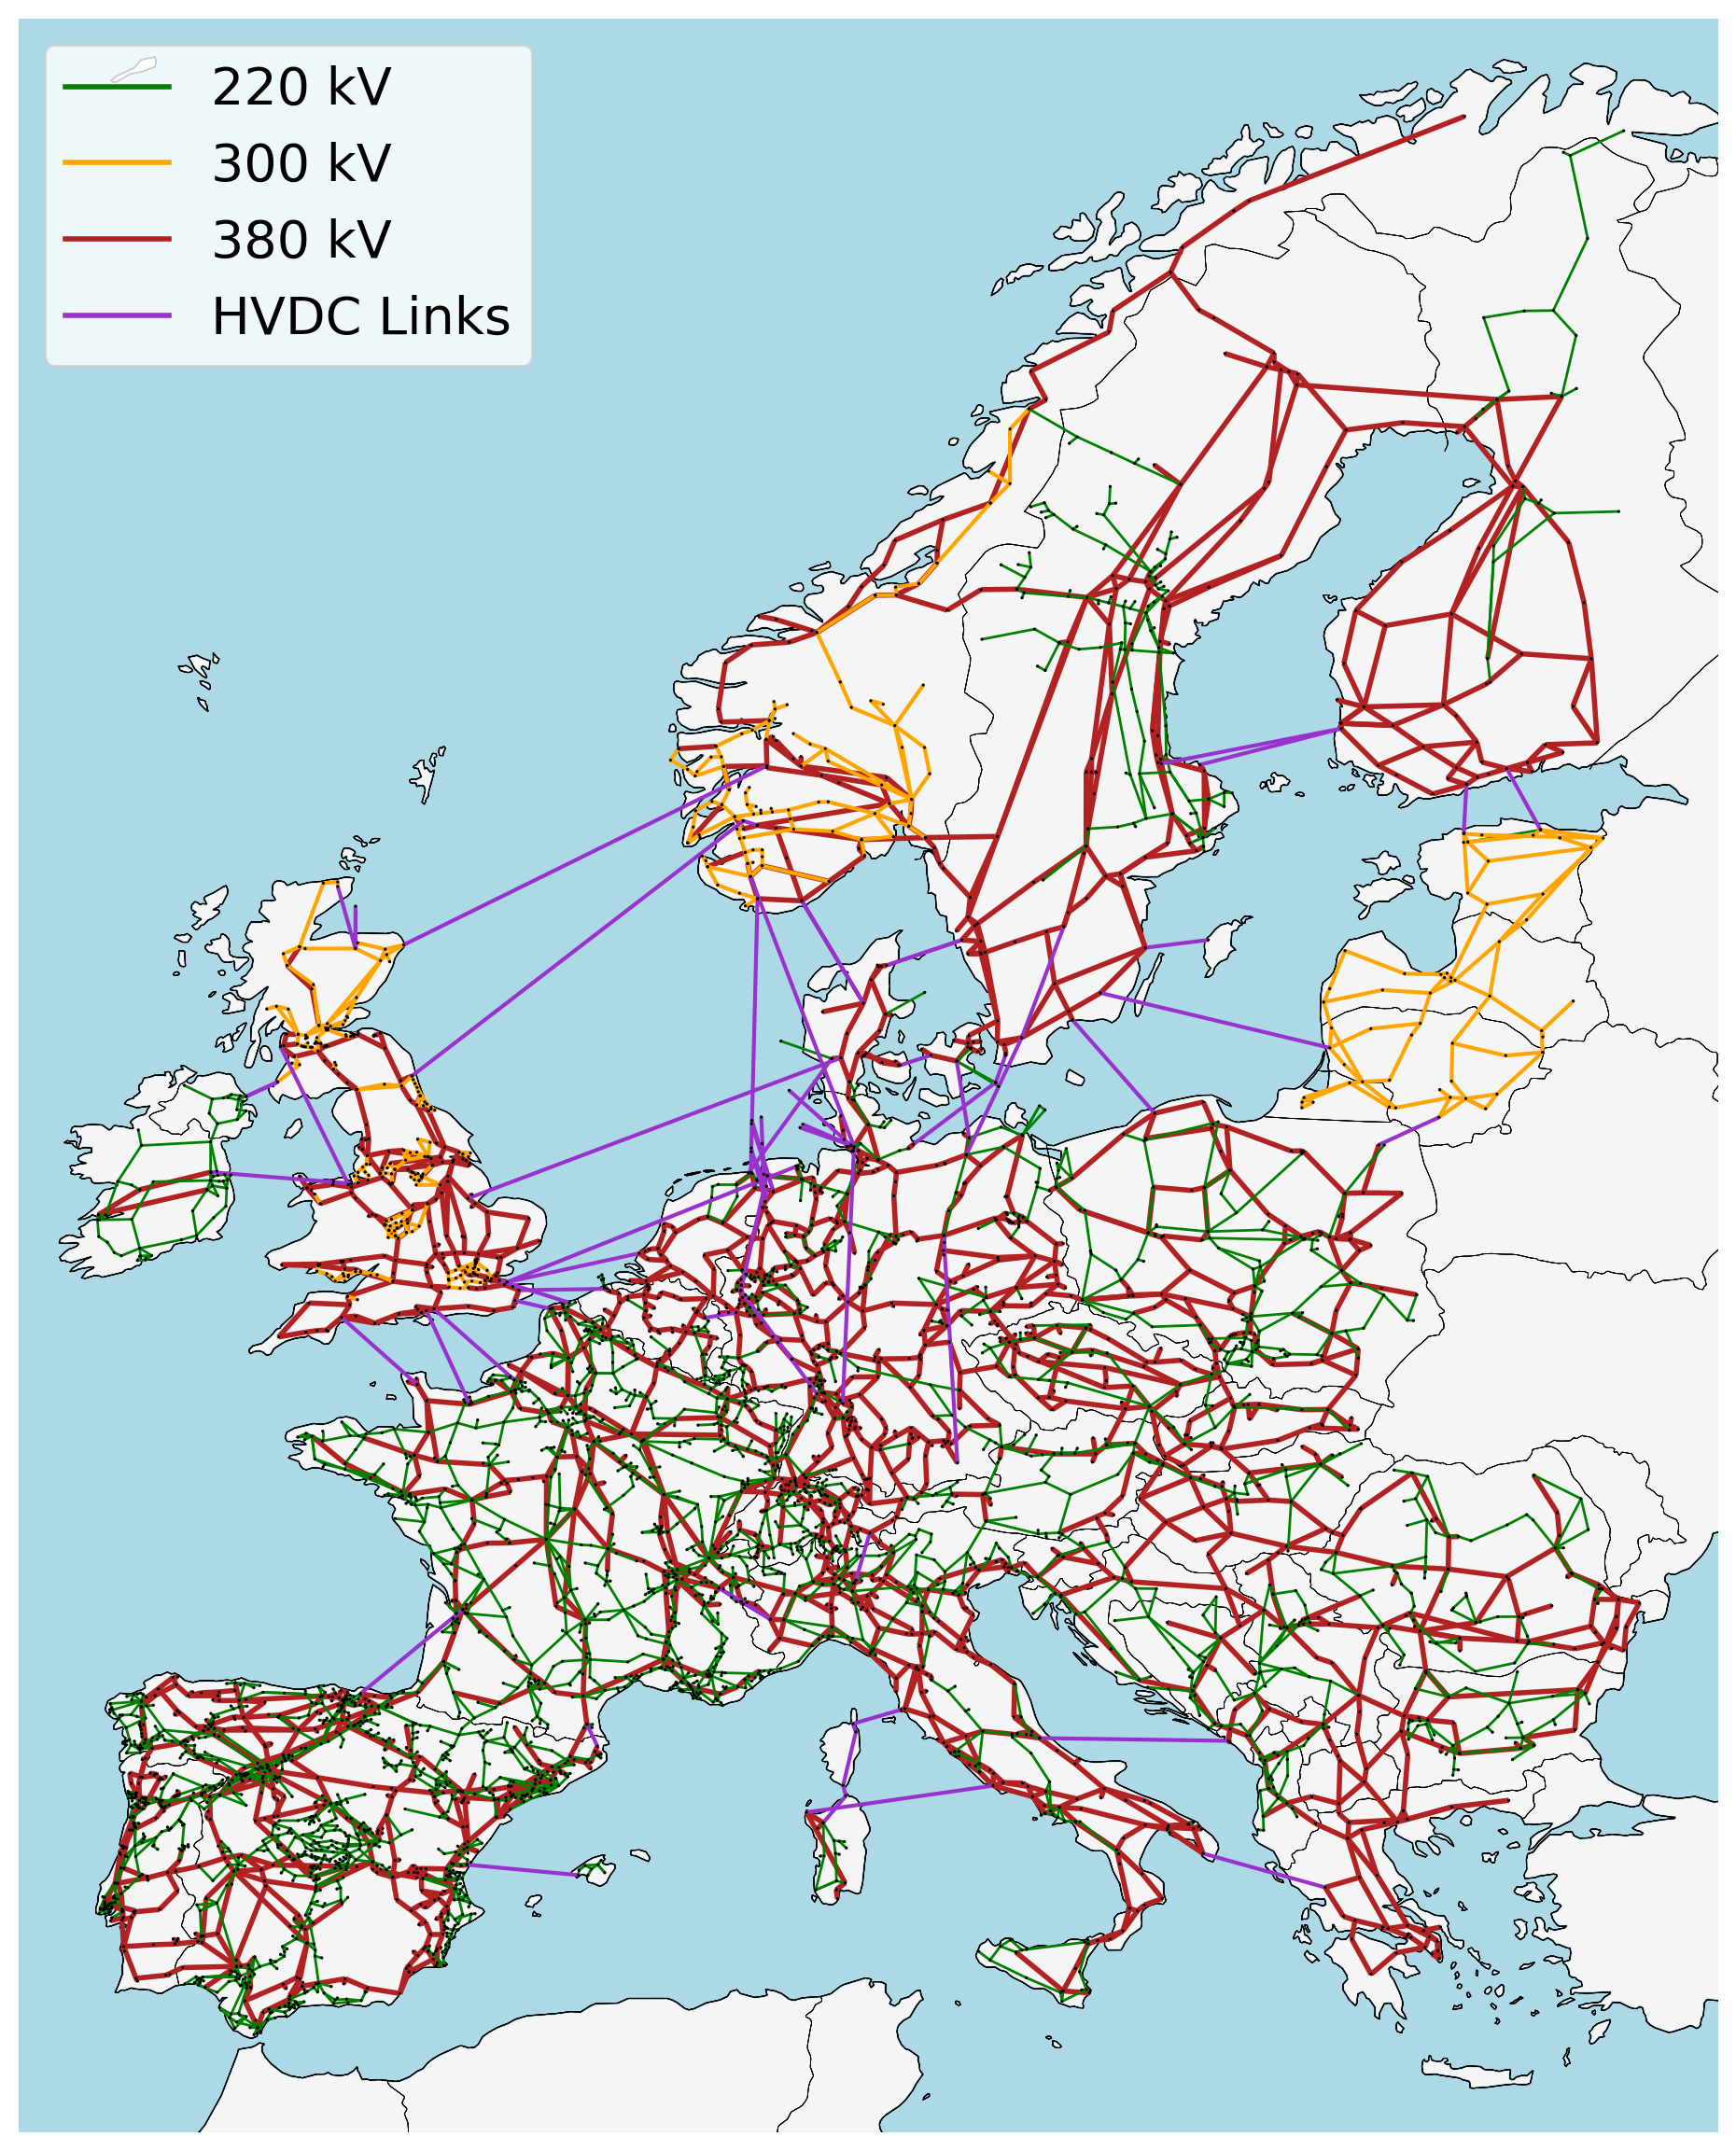
\includegraphics[width=7cm]{images/pypsa-eur-grid.png}

  {\footnotesize 
  \vspace{.1cm}
  Basic validation of grid model in 
  \hrefc{https://doi.org/10.1016/j.esr.2018.08.012}{Hörsch et al. (2018)}
  }
  \end{column}

  \begin{column}{7.5cm}
  {\small 
  \vspace{.3cm}
  \begin{itemize}
    \item Grid data contains AC lines at and above 220~kV voltage level, 
    all high voltage DC lines, and substations for the full 
    \hrefc{https://www.entsoe.eu/data/map/}{ENTSO-E area}.
    \item Grid data is collected by \hrefc{https://github.com/PyPSA/GridKit}{GridKit extraction} 
    of ENTSO-E interactive map
    \item Spatial resolution is
    \hrefc{https://pypsa-eur.readthedocs.io/en/latest/simplification/cluster_network.html}{adjustable}, 
    what allows spatial and topological analysis at different levels 
    (e.g. by transforming the transmission grid to a 380~kV only equivalent network).

  \end{itemize}
  }
  
  \end{column}
  \end{columns}

\end{frame}



\begin{frame}{Summary of data sources: power plants and technology costs}
 
  \begin{columns}[T]\

  \begin{column}{7.5cm}
    {\small 
    \begin{itemize}
      \item Existing generation fleet data is collected by cleaning, 
      standardizing and merging multiple power plant databases.
      
      \item The process is transparent and open-sourced via the 
      \hrefc{https://github.com/PyPSA/powerplantmatching}{powerplantmatching} package.
      The package provides all the important information about power plants in a ready-to-use format
      for the European power system. 
  
      \item Assumptions on energy system technologies (such as capital and operational costs, efficiencies, lifetimes, etc.) 
      are gathered from variety of open sources. The process is also open-sourced via the 
      \hrefc{https://github.com/PyPSA/technology-data}{technology-data} project. 
  
      \item Both tools are maintained by TU Berlin team.
  
    \end{itemize}
    }  
  \end{column}

  \begin{column}{7cm}

  \vspace{0.3cm}
  \centering

  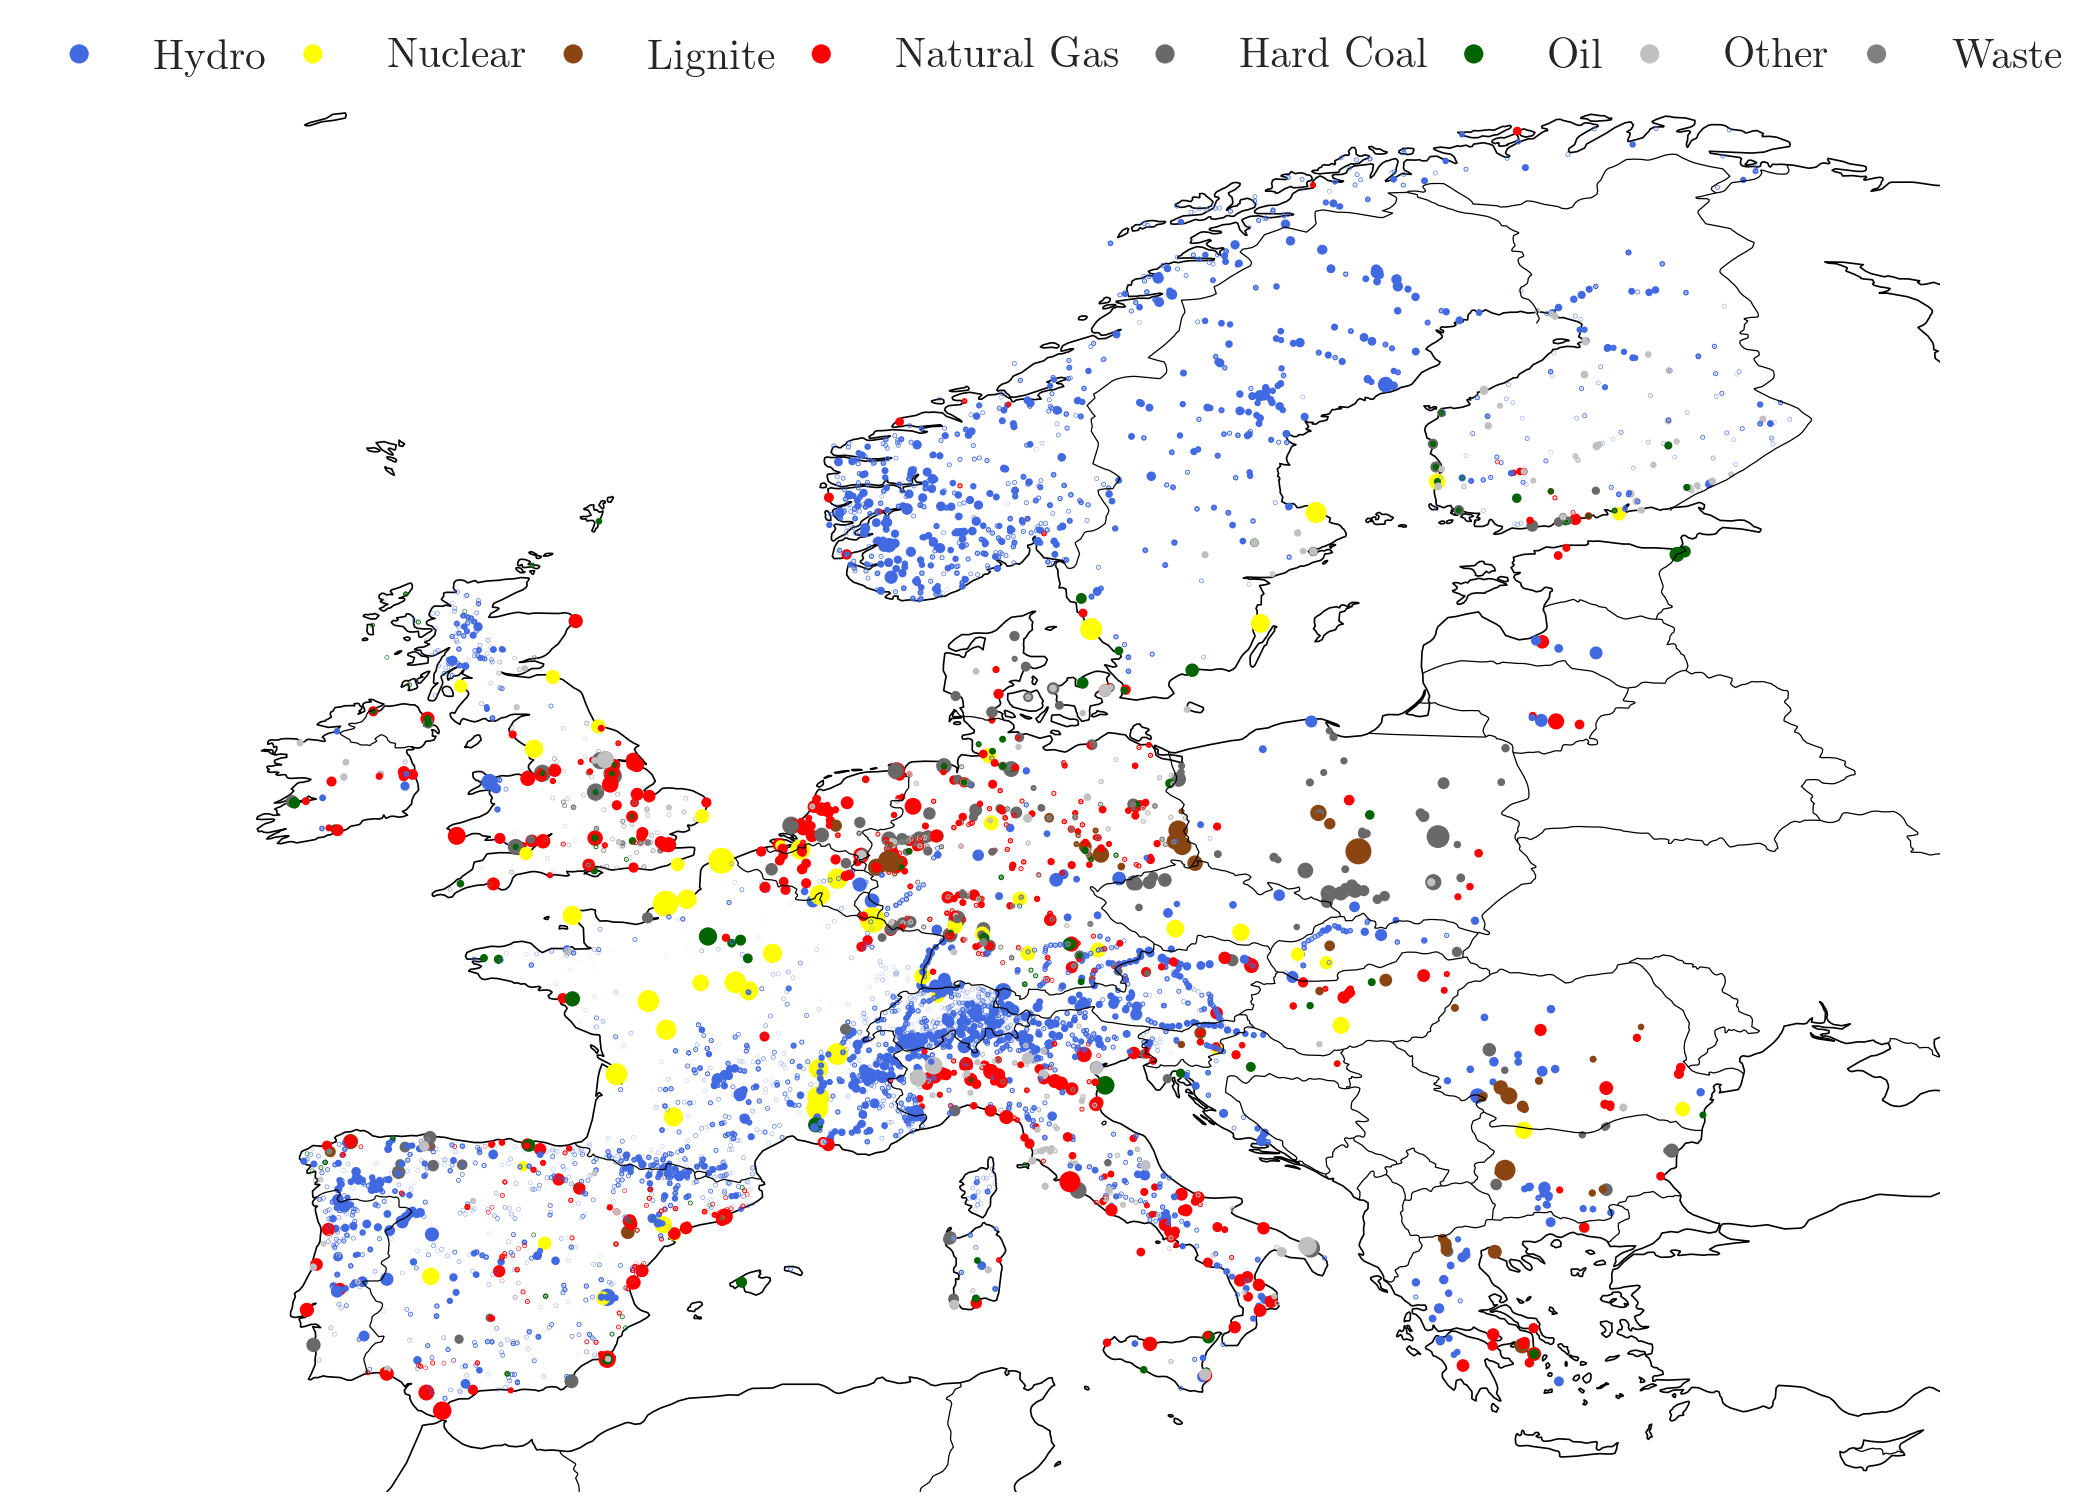
\includegraphics[width=7cm]{images/powerplantmatching.png}

  {\footnotesize 
  \vspace{0.1cm}
  A showcase example 
  of \hrefc{https://github.com/PyPSA/powerplantmatching}{powerplantmatching}
  }
  \end{column}
  \end{columns}

\end{frame}



\begin{frame}{Summary of data sources: renewable potentials and time series}
 
  \begin{columns}[T]
  \begin{column}{9cm}

  \vspace{0.3cm}
  \centering

  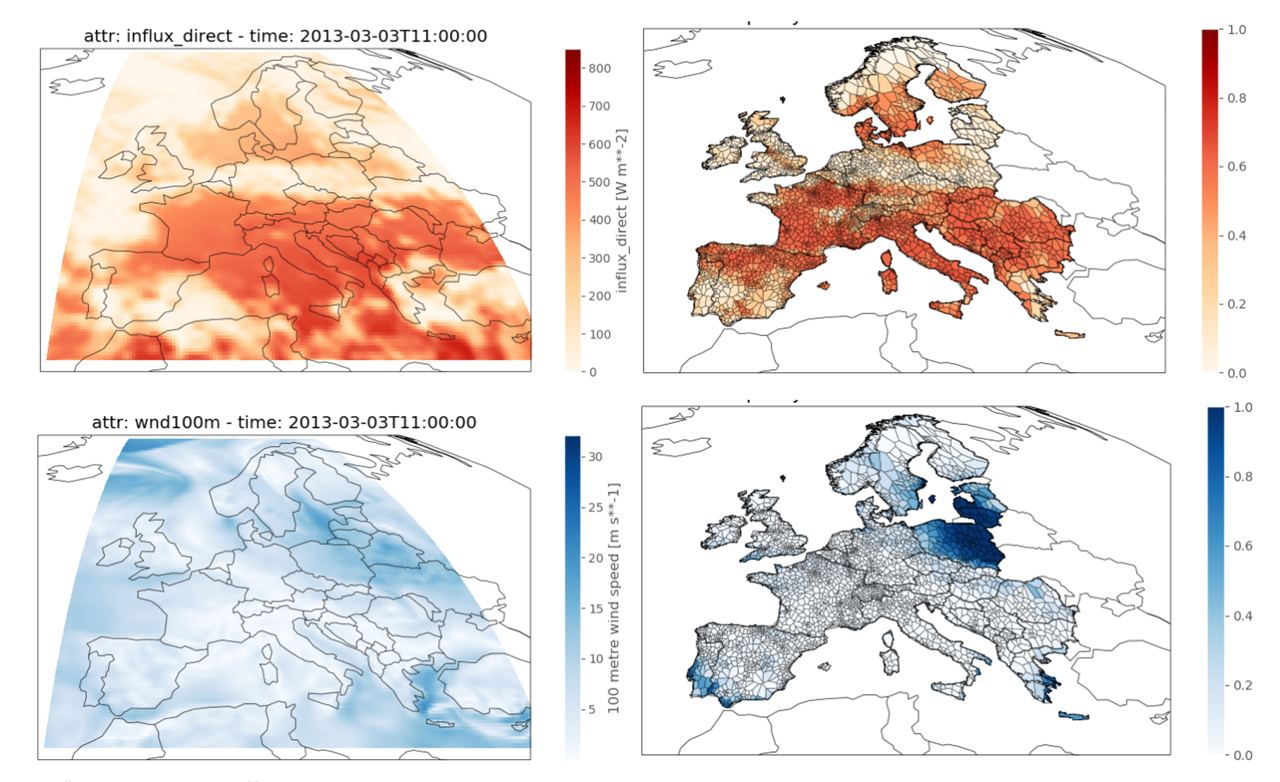
\includegraphics[width=9cm]{images/atlite.jpg}

  {\footnotesize 
  Converting weather data to energy system data with \hrefc{https://github.com/PyPSA/atlite}{atlite}
  }
  \end{column}

  \begin{column}{7cm}
  {\small 
  \begin{itemize}
    \item Renewable power potentials and generation profiles are processed by 
    the open-source \hrefc{https://github.com/PyPSA/atlite}{atlite} package, 
    which converts terabytes of weather data (like wind speeds, solar influx) 
    into the data for energy systems modelling.
    \item Geographic potentials for renewable energy are based on the
    \hrefc{https://github.com/FZJ-IEK3-VSA/glaes}{GLAES} framework. We gather and process
    datasets for land cover (CORINE2018), natural protection areas (NATURA2000),
    bathymetry (GEBCO2018) and \hrefc{https://pypsa-eur.readthedocs.io/en/latest/}{other} 
    to conduct own geospatial land availability analysis.
    \item The \alert{atlite} project is also maintained by TU Berlin team.

  \end{itemize}
  }
  
  \end{column}
  \end{columns}

\end{frame}


\begin{frame}{Other assumptions}

\begin{itemize}
  {\small 
\item Model is set to perform a \alert{perfect-foresight optimization} of investment 
and power dispatch decisions to meet electricity demand of the 24/7 consumers, 
as well as the demand of other consumers in the European electricity system for 2025 or 2030.
\item Electrical demand time-series is based on the 
\hrefc{https://open-power-system-data.org/}{OPSD project}. 
We assume the same demand profile per bidding zone for 2025 and 2030, as in the representative year 2013.
\item Similarly, we assume 2013 as the representative climate year for renewable in-feed.
\item Renewable expansion in the regional grid where 24/7 consumers are located is based on the 
\hrefc{https://energy.ec.europa.eu/topics/energy-strategy/national-energy-and-climate-plans-necps_en}{national energy and climate plans}.\footnote{{\scriptsize For Germany, we assume the 
\hrefc{https://www.bmwk.de/Redaktion/EN/Pressemitteilungen/2022/04/20220406-federal-minister-robert-habeck-says-easter-package-is-accelerator-for-renewable-energy.html}{Easter package}
to come into force as planned, i.e. RES cover 80\% of gross electricity consumption by 2030.}}
\item  National policies and decommissioning plans for coal and nuclear 
power plants are based on the 
\hrefc{https://beyond-coal.eu/}{Europe Beyond Coal}, 
and \hrefc{https://world-nuclear.org/}{world-nuclear.org} projects.
\item We assume price for EU ETS allowances to be 80~\euro/tCO$_2$ 
and 130~\euro/tCO$_2$ for 2025 and 2030, accordingly. The price for 
natural gas is assumed to be 35~\euro/MWh.\footnote{{\scriptsize Based on the price assumptions in the \hrefc{https://energy.ec.europa.eu/system/files/2022-05/SWD_2022_230_1_EN_autre_document_travail_service_part1_v3.pdf}{REPowerEU Plan}
issued by the European Commission in May 2022}}
}
\vspace{0.2cm}
\end{itemize}

\end{frame}


\begin{frame}{Technologies available for 24/7 consumers - 2025}
  
  {\scriptsize 

    \begin{tabular}{cccccccc}
      \hline
      Palette & Technology & CAPEX & FOM & VOM & Eff. & lifetime & Original reference \\
       &  & (overnight cost)  &  (\%/year) &  (€/MWh) & (per unit) & (years) & (\hrefc{https://github.com/PyPSA/technology-data}{technology data}) \\
      \hline
      1,2,3 & solar & 612 €/kW & 1.7 & 0.01 & - & 37.5 & \hrefc{https://ens.dk/en/our-services/projections-and-models/technology-data}{DEA}\\
      \hline
      1,2,3 & onshore wind & 1077 €/kW & 1.2 & 1.42 & - & 28.5 & \hrefc{https://ens.dk/en/our-services/projections-and-models/technology-data}{DEA}\\
      \hline
      1,2,3 & battery storage & 187 €/kWh & - & - & - & 22.5 & \hrefc{https://ens.dk/en/our-services/projections-and-models/technology-data}{DEA} \\
      \hline
      1,2,3  & battery inverter & 215 €/kW & 0.3 & - & 0.96  & 10.0 & \hrefc{https://ens.dk/en/our-services/projections-and-models/technology-data}{DEA} \\
      \hline
      2,3 & hydrogen storage\footnote{{\scriptsize Underground hydrogen storage in salt cavern}} 
                  & 2.5 €/kWh & 0 & 0 & - & 100.0 & \hrefc{https://ens.dk/en/our-services/projections-and-models/technology-data}{DEA} \\
      \hline
      2,3 & electrolysis & 550 €/kW & 2.0 & - & 0.67 & 27.5 & \hrefc{https://ens.dk/en/our-services/projections-and-models/technology-data}{DEA} \\
      \hline
      2,3 & fuel cell & 1200 €/kW & 5.0 & - & 0.50 & 10.0 & \hrefc{https://ens.dk/en/our-services/projections-and-models/technology-data}{DEA} \\
      \hline
      3 & NG Allam cycle\footnote{{\scriptsize Costs also include estimate of 40~€/ton for CO$_2$ transport \& sequestration.}} & 2760 €/kW & 14.8  & 3.2 & 0.54 & 30.0 &
      \hrefc{https://file.go.gov.sg/carbon-capture-utilisation-and-storage-decarbonisation-pathway-for-singapore-energy-and-chemical-sectors-pdf.pdf}{Navigant}, 
      \hrefc{https://netzeroamerica.princeton.edu/}{NZA}\\
      \hline
      3 & Advanced dispatchable
      & 10000 €/kW & 0 & 0 & 1.00 & 30.0 & own assumption \\
      \end{tabular}
  }

\end{frame}



\begin{frame}{Technologies available for 24/7 consumers - 2030}
  
  {\scriptsize 

    \begin{tabular}{cccccccc}
      \hline
      Palette & Technology & CAPEX & FOM & VOM & Eff. & lifetime & Original reference \\
       &  & (overnight cost)  &  (\%/year) &  (€/MWh) & (per unit) & (years) & (\hrefc{https://github.com/PyPSA/technology-data}{technology data}) \\
      \hline
      1,2,3 & solar & 492 €/kW & 2.0 & 0.01 & - & 40 & \hrefc{https://ens.dk/en/our-services/projections-and-models/technology-data}{DEA}\\
      \hline
      1,2,3 & onshore wind & 1035 €/kW & 1.2 & 1.35 & - & 30 & \hrefc{https://ens.dk/en/our-services/projections-and-models/technology-data}{DEA}\\
      \hline
      1,2,3 & battery storage & 142 €/kWh & - & - & - & 25.0 & \hrefc{https://ens.dk/en/our-services/projections-and-models/technology-data}{DEA} \\
      \hline
      1,2,3  & battery inverter & 160 €/kW & 0.3 & - & 0.96  & 10.0 & \hrefc{https://ens.dk/en/our-services/projections-and-models/technology-data}{DEA} \\
      \hline
      2,3 & hydrogen storage\footnote{{\scriptsize Underground hydrogen storage in salt cavern}} 
                  & 2.0 €/kWh & 0 & 0 & - & 100 & \hrefc{https://ens.dk/en/our-services/projections-and-models/technology-data}{DEA} \\
      \hline
      2,3 & electrolysis & 450 €/kW & 2.0 & - & 0.68 & 30.0 & \hrefc{https://ens.dk/en/our-services/projections-and-models/technology-data}{DEA} \\
      \hline
      2,3 & fuel cell & 1100 €/kW & 5.0 & - & 0.5 & 10.0 & \hrefc{https://ens.dk/en/our-services/projections-and-models/technology-data}{DEA} \\
      \hline
      3 & NG Allam cycle\footnote{{\scriptsize Costs also include estimate of 40~€/ton for CO$_2$ transport \& sequestration.}}  & 2600 €/kW & 14.8  & 3.2 & 0.54 & 30 &
      \hrefc{https://file.go.gov.sg/carbon-capture-utilisation-and-storage-decarbonisation-pathway-for-singapore-energy-and-chemical-sectors-pdf.pdf}{Navigant}, 
      \hrefc{https://netzeroamerica.princeton.edu/}{NZA}\\
      \hline
      3& Advanced dispatchable
      & 10000 €/kW & 0 & 0 & 1 & 30 & own assumption \\
      \end{tabular}
  }

\end{frame}


%---------------------------------------------
%---------------------------------------------
\section{Modelling results and analysis}


%----------------------------------

\begin{frame}{Scenario space}

  {\small
  The following section presents modelling results and related analysis. 
  For convenience, we start with a \alert{base scenario} 
  with the following setup:

    \quad{\bf Zone:} IE | DE | DK1 | NL \\
    \quad{\bf Technology palette:} 1 | 2 | 3 \\
    \quad{\bf Year:} 2025 \\ 
    \quad{\bf Participation rate:} 10\% of C\&I demand in a modelled zone \\
    \quad{\bf Demand profile}: baseload (flat) \\
  
  \vspace{0.3cm}
  Afterwards, we explore the scenario space further by implementing one-at-a-time 
  adjustments to the base scenario: \\
  (i) implementing year {\bf 2030}, \\
  (ii) implementing participation rate of {\bf 25\%}, \\ 
  (iii) implementing {\bf other types of demand profiles} for C\&I consumers.
  
  \vspace{0.3cm}
  For interested parties, we publish an \hrefc{https://doi.org/10.5281/zenodo.7180098}{online annex} 
  with a full pack of modelling results alongside this study. The annex 
  includes modelling results for all scenario combinations.
  }
  \end{frame}

%----------------------------------

\begin{frame}{Base scenario: Ireland -- Palette 1}

{\footnotesize
\vspace{0.3cm}

\begin{columns}[T]
\begin{column}{9cm}
\centering

\includegraphics[width=9.4cm]{../results/report/plots/10/2025/IE/p1/used.pdf}
\end{column}
\begin{column}{6cm}

\vspace{0.1cm}
A plot on the left shows the {\bf fraction of hourly demand met with carbon-free
electricity} depending on the procurement policy that C\&I consumers follow.

\vspace{0.3cm}
In the reference case, where C\&I consumers do not procure any resources,  
relying purely on grid purchases, \alert{only 61\%} of demand is met with CFE.

\vspace{0.3cm}
100\% RES -- the best case for the annual renewable matching policy -- 
results in 85\% fraction. Thus, \alert{CFE targets beyond 85\%} yield 
higher share of hourly demand met with CFE
than 100\% RES procurement policy.

\vspace{0.3cm}
When CFE target approaches 100\%, C\&I participants 
\alert{rely more on procured resources}.

\end{column}
\end{columns}
}
\source{Ireland -- Palette 1 -- 2025 -- 10\% -- baseload}
\end{frame}



\begin{frame}{Base scenario: Ireland -- Palette 1}

{\footnotesize
\vspace{0.3cm}

\begin{columns}[T]
\begin{column}{9cm}
\centering

\includegraphics[width=9.4cm]{../results/report/plots/10/2025/IE/p1/ci_emisrate.pdf}

\end{column}
\begin{column}{6cm}

\vspace{0.1cm}
Next, we investigate how the choice of a procurement policy affects the {\bf average emissions 
rate} of 24/7 participating C\&I consumers.

\vspace{0.3cm}
Already in 2025, Ireland has a moderately clean electricity system: 
the C\&I emission rate in the reference case is at 138~kg/MWh.

\vspace{0.3cm}
100\% annual matching with renewable energy reduces the 
C\&I emission rate to 53 kg/MWh.

\vspace{0.3cm}
When actively matching the carbon-free electricity and the load with 
24/7 procurement, C\&I participants can achieve \alert{lower emission 
rates than with the 100\% RES policy} with CFE targets beyond 85\%. 
As CFE target is tightened further, average emissions \alert{drop to zero}.

\end{column}
\end{columns}
}
\source{Ireland -- Palette 1 -- 2025 -- 10\% -- baseload}
\end{frame}



\begin{frame}{Base scenario: Ireland -- Palette 1}

  {\footnotesize
  \vspace{0.3cm}
  
  \begin{columns}[T]
  \begin{column}{9cm}
  \centering
  
  \includegraphics[width=9.4cm]{../results/report/plots/10/2025/IE/p1/ci_capacity.pdf}
  \end{column}
  \begin{column}{6cm}
  
  \vspace{0.1cm}
  If we now turn to the {\bf portfolio capacity} procured by 
  C\&I consumers, we see that at this level of participation
  (10\% of C\&I load in Ireland is at 220~MW), the 100\% RES policy can be 
  me by procuring near to 1.5~GW of onshore wind and solar generators.
  
  \vspace{0.3cm}
  In this scenario, hourly matching renewable generation and the 24/7 participating load
  requires a \alert{much bigger portfolio} of renewable generators than the 
  100\% RES policy. 

  \vspace{0.3cm}
  Also, above 85\% 24/7 procurement sees \alert{battery storage} enter the portfolio  mix.
  
  \vspace{0.3cm}
  Note that for 80\% CFE, 24/7 participating C\&I consumers procure less 
  capacity than for 100\% RES policy, as it relies more on grid imports.

  \end{column}
  \end{columns}
  }
  \source{Ireland -- Palette 1 -- 2025 -- 10\% -- baseload}
  \end{frame}



\begin{frame}{Base scenario: Ireland -- Palette 1}

    {\footnotesize
    \vspace{0.3cm}
    
    \begin{columns}[T]
    \begin{column}{9cm}
    \centering
    
    \includegraphics[width=9.4cm]{../results/report/plots/10/2025/IE/p1/ci_costandrev.pdf}
    \end{column}
    \begin{column}{6cm}
    
    \vspace{0.1cm}
    It is also interesting to look at the {\bf breakdown of costs associated with
    a procurement policy} that C\&I consumers choose. 
    
    \vspace{0.3cm}
    Note that revenues from selling the excess electricity to the regional grid 
    (dark green) at market prices can be treated as "negative costs" and 
    subtracted from the net procurement cost.

    \vspace{0.3cm}
    A CFE target of 90-95\% can be achieved at a small cost premium to 100\% 
    annual renewable matching with solar, wind and batteries. However,
    what stands out in the plot is the rapid increase of procurement costs  
    for high CFE targets. For example, 98\% CFE target has 
    cost premium of only 55\% over 100\% annual renewable matching; while
    \alert{the last 2\% of hourly CFE matching more than doubles the 
    cost}.
  
    \end{column}
    \end{columns}
    }
    \source{Ireland -- Palette 1 -- 2025 -- 10\% -- baseload}
    \end{frame}



\begin{frame}{Base scenario: Ireland -- Palette 2}

    {\footnotesize
  
    \begin{columns}
    \begin{column}{7cm}
    \centering
    \includegraphics[width=7.5cm]{../results/report/plots/10/2025/IE/p2/ci_capacity.pdf}
    \end{column}
  
    \begin{column}{8cm}
    \centering
    \includegraphics[width=7.5cm]{../results/report/plots/10/2025/IE/p2/ci_costandrev.pdf}
    \end{column}
  
    \end{columns}
  
    \begin{columns}
    \begin{column}{15cm}
    If we look at the results for the technological {\bf Palette 2} -- 
    when C\&I consumers have an access to the long-duration energy storage (LDES) --
    we see a different picture. The portfolio of renewable capacity 
    C\&I consumers for the 100\% CFE target is not much larger 
    than for 100\% RES (see the left panel). The LDES system helps to align the load 
    with the generation of procured variable renewable resources. 
    In the right panel, we can see that a LDES system (here 2.5~€/kWh 
    hydrogen storage in caverns) can \alert{significantly limit the procurement cost
    increase} at high CFE targets. In this scenario, 
    100\% CFE costs only 50\% more than a 100\% RES policy.

    \end{column}
    \end{columns}
    }
  
    \source{Ireland -- Palette 2 -- 2025 -- 10\% -- baseload}
\end{frame}



\begin{frame}{Base scenario: Ireland -- Palette 3}

  {\footnotesize

  \begin{columns}
  \begin{column}{7cm}
  \centering
  \includegraphics[width=7.5cm]{../results/report/plots/10/2025/IE/p3/ci_capacity.pdf}
  \end{column}

  \begin{column}{8cm}
  \centering
  \includegraphics[width=7.5cm]{../results/report/plots/10/2025/IE/p3/ci_costandrev.pdf}
  \end{column}

  \end{columns}

  \begin{columns}
  \begin{column}{15cm}
  Finally, the results for technological {\bf Palette 3} scenario show that 24/7 procurement
  can create a market for and benefit from the advanced technologies such as 
  NG Allam Cycle generator with carbon capture and sequestration or 
  advanced geothermal systems. 
  In the case of Ireland, NG Allam Cycle generator is added to the 
  procured portfolio. The clean dispatchable technology \alert{further limits 
  the hourly CFE cost premium} above annual renewable matching. 
  Inclusion of clean firm generation also reduces storage requirements.
  \end{column}
  \end{columns}
  }

  \source{Ireland -- Palette 3 -- 2025 -- 10\% -- baseload}
\end{frame}

%----- base scenario, system effects


\begin{frame}{Base scenario: Ireland -- Palette 3}

  {\footnotesize
  \vspace{0.1cm}
  
  \begin{columns}[T]
  \begin{column}{9cm}
  \centering
  
  \includegraphics[width=9.4cm]{../results/report/plots/10/2025/IE/p3/zone_emissions.pdf}
  
  \end{column}
  \begin{column}{6cm}
  
  \vspace{0.1cm}
  In the next step, we explore how the 24/7 procurement affects the 
  rest of the electricity system. The plot on the left shows
  {\bf CO$_2$~emissions in the local region} of 24/7 participating 
  consumers -- Ireland.
  
  \vspace{0.1cm}
  Without any procurement, the model estimates 
  Irish power sector carbon emissions to be at the level of 3.5~MtCO$_2$
  (for comparison, 
  \hrefc{https://www.seai.ie/data-and-insights/seai-statistics/key-statistics/co2/}{seai.ie}
  reports this value to be at 8.4~MtCO$_2$ in 2020, with a strong decreasing trend).

  \vspace{0.1cm}
  100\% annual renewable matching can deliver greater system-level CO$_2$ emissions
  reductions than lower CFE scores. 100\% RES reduces emissions in Ireland by 
  ca. 0.6~MtCO$_2$ per year (at 10\% participation rate).
  
  \vspace{0.1cm}
  However, beyond 85\% CFE targets, 24/7 hourly matching achieves
  \alert{greater emissions reductions} than 100\% RES.

  \end{column}
  \end{columns}
  }
  \source{Ireland -- Palette 3 -- 2025 -- 10\% -- baseload}
\end{frame}

%----------------------------------------
%Base scenario - other countries

\begin{frame}{Base scenario: other regions}
  \centering
  
  Results for other regions in Europe where C\&I load commits to voluntary  \\ 
  CFE procurement 
  show \alert{similar trends.} \\ 
  
  \vspace{0.3cm}
  However, each region has a \alert{unique set of characteristics} 
  that depend on local resources, renewable potentials,
  national energy and climate policies, degree of interconnections, etc.

  \vspace{0.3cm}
  Despite regional differences, the dynamics of 24/7 CFE procurement, \\
  observed in the example of Ireland, repeat in other regions.

\end{frame}


%---------------------------------------- Portfolio and Costs
%----------------------------------------

\begin{frame}{Google DC locations setup: Portfolio breakdown}

  \centering
  {\footnotesize
  The optimal procurement strategy adjusts in all locations \\ 
  in presense of the \alert{spatial} and \alert{temporal} load management systems. 
  }
  
\includegraphics[height=6.3cm]{../results/final-EU-1H-GoogleDC-allflex/plots/2025/EU/p1/cfe100/capacity.pdf}

\source{EU -- 24/7 CFE 100\% -- Palette 1 -- 2025 -- 100~MW}
\end{frame}


\begin{frame}{Google DC locations setup: 24/7 cost breakdown}

  \centering
  {\footnotesize
  The \alert{cost breakdown} shows the average costs of meeting demand with the policy, including grid electricity consumption costs netted by revenue selling to the grid.
  100\% hourly matching target is costly with palette~1 technologies. Co-optimized utilization of spatial and temporal load flexibility \alert{considerably reduces} the costs.
  }

\vspace{-0.2cm} 
\includegraphics[height=6.3cm]{../results/final-EU-1H-GoogleDC-allflex/plots/2025/EU/p1/cfe100/ci_costandrev.pdf}

\source{EU -- 24/7 CFE 100\% -- Palette 1 -- 2025 -- 100~MW}
\end{frame}


\begin{frame}{Alternative DC locations setup: Portfolio breakdown}

  \centering
  {\footnotesize
  The optimal procurement strategy adjusts in all locations \\ 
  in presense of the \alert{spatial} and \alert{temporal} load management systems. 
  }

\includegraphics[height=6.3cm]{../results/final-EU-1H-BroadDC-allflex/plots/2025/EU/p1/cfe100/capacity.pdf}

\source{EU -- 24/7 CFE 100\% -- Palette 1 -- 2025 -- 100~MW}
\end{frame}


\begin{frame}{Alternative DC locations setup: 24/7 cost breakdown}

  \centering
  {\footnotesize
  The \alert{cost breakdown} shows the average costs of meeting demand with the policy, including grid electricity consumption costs netted by revenue selling to the grid.
  100\% hourly matching target is costly with palette~1 technologies. Co-optimized utilization of spatial and temporal load flexibility \alert{considerably reduces} the costs.
  }

\vspace{-0.2cm}   
\includegraphics[height=6.3cm]{../results/final-EU-1H-BroadDC-allflex/plots/2025/EU/p1/cfe100/ci_costandrev.pdf}

\source{EU -- 24/7 CFE 100\% -- Palette 1 -- 2025 -- 100~MW}
\end{frame}


\begin{frame}{24/7 CFE procurement net annual costs comparison}

  \centering
  {\footnotesize
  Google DC locations (left) and alternative DC locations (right).
  }
  \vspace{.5cm}
  
  \begin{columns}
  \begin{column}{7cm}
  \centering
  \includegraphics[width=7.5cm]{../results/final-EU-1H-GoogleDC-allflex/plots/2025/EU/p1/cfe100/ci_abs_costs.pdf}
  \end{column}
  
  \begin{column}{8cm}
    \centering
    \includegraphics[width=7.5cm]{../results/final-EU-1H-BroadDC-allflex/plots/2025/EU/p1/cfe100/ci_abs_costs.pdf}
    \end{column}
  \end{columns}
  
  \source{EU -- 24/7 CFE 100\% -- Palette 1 -- 2025 -- 100~MW}
  
\end{frame}


\begin{frame}{Google DC locations setup: spatial flexibility only}
  
  \centering

  {\footnotesize
  The cost breakdown [\euro/MWh] (left) and the net 24/7 CFE procurement annual costs [\euro/a] (right)
  }
  \vspace{.5cm}

  \begin{columns}
    \begin{column}{8cm}
    \centering
    \includegraphics[width=8.5cm]{../results/final-EU-1H-GoogleDC-spatial/plots/2025/EU/p1/cfe100/ci_costandrev.pdf}
    \end{column}
    
    \begin{column}{8cm}
      \centering
      \includegraphics[width=7cm]{../results/final-EU-1H-GoogleDC-spatial/plots/2025/EU/p1/cfe100/ci_abs_costs.pdf}
      \end{column}
    \end{columns}

\source{EU -- 24/7 CFE 100\% -- Palette 1 -- 2025 -- 100~MW}
\end{frame}


\begin{frame}{Google DC locations setup: temporal flexibility only}

  \centering

  {\footnotesize
  The cost breakdown [\euro/MWh] (left) and the net 24/7 CFE procurement annual costs [\euro/a] (right)
  }
  \vspace{.5cm}
  
  \begin{columns}
    \begin{column}{8cm}
    \centering
    \includegraphics[width=8.5cm]{../results/final-EU-1H-GoogleDC-temporal/plots/2025/EU/p1/cfe100/ci_costandrev.pdf}
    \end{column}
    
    \begin{column}{8cm}
      \centering
      \includegraphics[width=7cm]{../results/final-EU-1H-GoogleDC-temporal/plots/2025/EU/p1/cfe100/ci_abs_costs.pdf}
      \end{column}
    \end{columns}

\source{EU -- 24/7 CFE 100\% -- Palette 1 -- 2025 -- 100~MW}
\end{frame}


\begin{frame}{Google DC locations setup: spatial flexibility only}

  \centering

  {\footnotesize
  The cost breakdown [\euro/MWh] (left) and the net 24/7 CFE procurement annual costs [\euro/a] (right)
  }
  \vspace{.5cm}
  
  \begin{columns}
    \begin{column}{8cm}
    \centering
    \includegraphics[width=8.5cm]{../results/final-EU-1H-GoogleDC-spatial/plots/2025/EU/p2/cfe100/ci_costandrev.pdf}
    \end{column}
    
    \begin{column}{8cm}
      \centering
      \includegraphics[width=7cm]{../results/final-EU-1H-GoogleDC-spatial/plots/2025/EU/p2/cfe100/ci_abs_costs.pdf}
      \end{column}
    \end{columns}

\source{EU -- 24/7 CFE 100\% -- Palette 2 -- 2025 -- 100~MW}
\end{frame}


\begin{frame}{Google DC locations setup: temporal flexibility only}

  \centering

  {\footnotesize
  The cost breakdown [\euro/MWh] (left) and the net 24/7 CFE procurement annual costs [\euro/a] (right)
  }
  \vspace{.5cm}
  
  \begin{columns}
    \begin{column}{8cm}
    \centering
    \includegraphics[width=8.5cm]{../results/final-EU-1H-GoogleDC-temporal/plots/2025/EU/p2/cfe100/ci_costandrev.pdf}
    \end{column}
    
    \begin{column}{8cm}
      \centering
      \includegraphics[width=7cm]{../results/final-EU-1H-GoogleDC-temporal/plots/2025/EU/p2/cfe100/ci_abs_costs.pdf}
      \end{column}
    \end{columns}

\source{EU -- 24/7 CFE 100\% -- Palette 2 -- 2025 -- 100~MW}
\end{frame}


%----------------------------------------
%----------------------------------------
\section*{Economically efficient redistribution of data center loads}


\begin{frame}{Re-disribution of loads for co-optimised space-time flexibility utilisation \\
  DC in \{IE, DK, FR, FI, PT\} -- Tech-P1 -- CFE95\% (left), CFE100\% (right)}

  \begin{columns}[T]
  \begin{column}{6cm}
    \centering
    \includegraphics[width=6cm]{../results/final-EU-1H-BroadDC-allflex/plots/2025/EU/p1/cfe95/utilization_dc/utilization_dc.pdf}
  \end{column}

  \begin{column}{6cm}
    \centering
    \includegraphics[width=6cm]{../results/final-EU-1H-BroadDC-allflex/plots/2025/EU/p1/cfe100/utilization_dc/utilization_dc.pdf}  
  \end{column}
  \end{columns}

\end{frame}


\begin{frame}{Re-disribution of loads for co-optimised space-time flexibility utilisation \\
  DC in \{IE, DK, FR, FI, PT\} -- Tech-P2 -- CFE95\% (left), CFE100\% (right)}

  \begin{columns}[T]
  \begin{column}{6cm}
    \centering
    \includegraphics[width=6cm]{../results/final-EU-1H-BroadDC-allflex/plots/2025/EU/p2/cfe95/utilization_dc/utilization_dc.pdf}
  \end{column}

  \begin{column}{6cm}
    \centering
    \includegraphics[width=6cm]{../results/final-EU-1H-BroadDC-allflex/plots/2025/EU/p2/cfe100/utilization_dc/utilization_dc.pdf}  
  \end{column}
  \end{columns}

\end{frame}

%%%%%%%%%%%%%%%%%%%%%%% explanation


\begin{frame}{Hourly CFE score of supply from grid -- PT 2025}
  \vspace{.5cm}
  \includegraphics[height=5.5cm]{../results/final-EU-1H-BroadDC-allflex/plots/2025/EU/p1/cfe100/heatmaps/0_GridCFE_PT1 0.pdf}
\end{frame}


\begin{frame}{Co-optimized spatial \& temporal flexibility utilization \\
  Temporal load shifts for PT data center with f=40\%, CFE95\%}

  \vspace{.3cm}
  
  \centering
  \includegraphics[height=5.5cm]{../results/final-EU-1H-BroadDC-allflex/plots/2025/EU/p1/cfe95/heatmaps/40_temporal_shift_lisbon.pdf}

  \vspace{.3cm}

\end{frame}


\begin{frame}{Co-optimized spatial \& temporal flexibility utilization \\
  Spatial load shifts for PT data center with f=40\%, CFE95\%}

  \vspace{.3cm}
  
  \centering
  \includegraphics[height=5.5cm]{../results/final-EU-1H-BroadDC-allflex/plots/2025/EU/p1/cfe95/heatmaps/40_spatial_shift_lisbon.pdf}

  \vspace{.3cm}

\end{frame}


\begin{frame}{Co-optimized spatial \& temporal flexibility utilization \\
  Spatial load shifts for PT data center with f=40\%, CFE100\%}

  \vspace{.3cm}
  
  \centering
  \includegraphics[height=5.5cm]{../results/final-EU-1H-BroadDC-allflex/plots/2025/EU/p1/cfe100/heatmaps/40_spatial_shift_lisbon.pdf}

  \vspace{.3cm}

\end{frame}

%%% Dublin & Frederica


\begin{frame}{Hourly CFE score of supply from grid -- IE 2025}
  \vspace{.5cm}
  \includegraphics[height=5.5cm]{../results/final-EU-1H-GoogleDC-allflex/plots/2025/EU/p1/cfe100/heatmaps/0_GridCFE_IE5 0.pdf}
\end{frame}


\begin{frame}{Hourly CFE score of supply from grid -- DK 2025}
  \vspace{.5cm}
  \includegraphics[height=5.5cm]{../results/final-EU-1H-GoogleDC-allflex/plots/2025/EU/p1/cfe100/heatmaps/0_GridCFE_DK1 0.pdf}
\end{frame}




\begin{frame}{Co-optimized spatial \& temporal flexibility utilization \\
  Spatial load shifts for IE data center with f=40\%, CFE100\%}

  \vspace{.3cm}
  
  \centering
  \includegraphics[height=5.5cm]{../results/final-EU-1H-BroadDC-allflex/plots/2025/EU/p1/cfe100/heatmaps/40_spatial_shift_dublin.pdf}

  \vspace{.3cm}

\end{frame}


\begin{frame}{Co-optimized spatial \& temporal flexibility utilization \\
  Spatial load shifts for DK data center with f=40\%, CFE100\%}

  \vspace{.3cm}
  
  \centering
  \includegraphics[height=5.5cm]{../results/final-EU-1H-BroadDC-allflex/plots/2025/EU/p1/cfe100/heatmaps/40_spatial_shift_frederica.pdf}

  {\scriptsize
  Results for tech-P1: solar PV, onshore wind, battery storage \\
  NB average capacity factor for onshore wind in Denmark is slighly above the value Ireland
  }

\end{frame}


\begin{frame}{Co-optimized spatial \& temporal flexibility utilization \\
  Spatial load shifts for DK data center with f=40\%, CFE100\%}

  \vspace{.3cm}
  
  \centering
  \includegraphics[height=5.5cm]{../results/final-EU-1H-BroadDC-allflex/plots/2025/EU/p2/cfe100/heatmaps/40_spatial_shift_frederica.pdf}

  {\scriptsize
  Note an increase of average load of DC located in Denmark, once LDES is added to the tehcnology mix. \\
  LDES helps harvesting best wind resources in DK1 zone, 
  which facilitates \alert{economically efficient redistribution} of DC loads.
  }
\end{frame}


%----------------------------------------
%----------------------------------------
\section{Technical summary}


\begin{frame}{Interplay of space-time load-shifting flexibility for data centers \& \\ 
  24/7 carbon-free electricity procurement 1/3}

  {\footnotesize
  \begin{itemize}

    \item [Spatial load management mechanisms] Shifting workloads across locations enables \\
          (i) taking advantage from \alert{difference in weather conditions} for distant DCs \\
          (ii) taking advantage from \alert{difference in local resources}, i.e., location-specific average CFs for RES technologies
    
    \item [Temporal load management mechanisms] Shifting workloads across time enables\\ 
          (i) \alert{execution of flexible loads in 'greener' times}, i.e., optimize consumption as function of the local grid's carbon intensity (CFE targets $<100\%$) \\
          (ii) facilitating \alert{better utilization of locally procured resources}

    \item [24/7 CFE procurement] Impacts on optimal procurement strategy:\\ 
          (i) Procurement strategy adjusts in presense of the spatial and temporal load management systems \\ 
          (ii) Co-optimized utilization of spatial and temporal load flexibility \alert{reduces and re-allocates RES portfolio} needed for achieving 24/7 procurement goals \\
          (iii) Spatial load management enables reduction of both locally procured generation and battery storage portfolio, while temporal load management mainly reduces the needs for battery storage \\

  \end{itemize}
  }
\end{frame}


\begin{frame}{Interplay of space-time load-shifting flexibility for data centers \& \\ 
  24/7 carbon-free electricity procurement 2/3}

{\footnotesize
\begin{itemize}

  \item [24/7 CFE costs] Impacts on costs of meeting demand with the CFE policy:\\ 
        (i) Co-optimized utilization of spatial and temporal load flexibility \alert{considerably reduces the costs of achieving 24/7 CFE goals} \\
        (ii) [CFE target 100\%] For tech palette of wind, solar PV and battery storage, the values of load management mechanisms are in a range of 6--9 (spatial) to 1 (temporal) \\
        (iii) [CFE target 100\%] If LDES is available on a market (here at 2.5 €/kWh hydrogen storage), the range is at 2--2.5~(spatial) to 1~(temporal) \\
        (iv) With LDES, data center operators can maximise utilization of local resources

  \item Operational aspects:\\
        (i) Optimal utilization of spatial load flexibility can have 
        \alert {a clear daily \& seasonal profiles} (driven by diff. in local resources), 
        as well as a \alert{stochastic profile} (driven by diff. in weather conditions -- vertical stripes in utilization heatmaps) \\
        (ii) Optimal utilization of temporal load flexibility can have \alert{unimodal- and bimodal distributions} (driven by the shape CFE profile in a local grid)


\end{itemize}
}

\end{frame}


\begin{frame}{Interplay of space-time load-shifting flexibility for data centers \& \\ 
  24/7 carbon-free electricity procurement 3/3}

{\footnotesize
\begin{itemize}

  \item Average utilization of data centers:\\
        (i) Spatial \& temporal load management mechanisms facilitate \alert{economically efficient redistribution} of data center loads \\
        (ii) Average capacity factors of data centers generally stay within a narrow range \\
        (iii) 24/7 CFE targets and technological palette notably affect the optimal average capacity factors.

  \item Other benefits of spatial \& temporal load management: \\
        (i) \alert{Reduction of RES curtailment} \\
        (ii) First movers implementing spatial \& temporal flexibilities will \alert{pave the way for followers} by incremental innovation and learning-by-doing \\
        (iii) .. and make \alert{simpler achieving clean energy procurement goals for others} who do not have flexibility options, via e.g., 
        direct (selling) or indirect (lower demand) ways for reducing prices for Guarantees of Origin.

\end{itemize}
}

\end{frame}


%----------------------------------------
%----------------------------------------
\section{Conclusions and project outlook}

{\small
\begin{frame}{Conclusions}

   \noindent\fbox{%
   \parbox{\textwidth}{%
     {\bf Conclusion 1:} 24/7~carbon-free energy (CFE) procurement leads to 
     \alert{lower emissions for both the buyer and the system},
     as well as reducing the needs for flexibility in the rest of the system.  
   }}

   \noindent\fbox{%
   \parbox{\textwidth}{%
     {\bf Conclusion 2:} Reaching CFE for 90-95\% of the time can be done with only a \alert{small cost premium}
      compared to annually matching 100\% renewable energy. 
      90-95\% CFE can be met by supplementing wind and solar with battery storage.
   }}

   \noindent\fbox{%
   \parbox{\textwidth}{%
     {\bf Conclusion 3:} Reaching 100\% CFE target is possible but costly with existing renewable 
     and storage technologies, with \alert{costs increasing rapidly above 95\%}.
   }}

   \noindent\fbox{%
   \parbox{\textwidth}{%
     {\bf Conclusion 4:} 100\% CFE target could have a \alert{much smaller cost premium} if long duration storage or 
      clean dispatchable technologies like advanced geothermal are available.
   }}

   \noindent\fbox{%
   \parbox{\textwidth}{%
     {\bf Conclusion 5:} 24/7~CFE procurement would create an early market for the advanced technologies,
     stimulating innovation and learning from which the \alert{whole electricity system would benefit}.
    }}

\end{frame}



\begin{frame}{Project outlook}
  
  This project will continue analysing the impact of 24/7~CFE procurement in Europe until March 2024. \\
  In the following study, we consider deepen the analysis by examining the following:

    \begin{itemize}
      \item The impacts of \alert{parametric uncertainties} and corresponding assumptions when constructing the model of 
      the European energy system. These include: \\
      \quad (i) Weather year realizations; \\
      \quad (ii) Scenarios for carbon price developments in the EU ETS; \\
      \quad (iii) Scenarios for inter-connector capacities based on the TYNDP or free optimization; \\
      \quad (iv) Scenarios for expansion of electric vehicles, heat pumps, industry electrification; \\
      \quad (v) Prices for primary energy carriers. 
      \item In addition, the modelling will use a \alert{higher-resolution grid} model,
       so that transmission network impacts can be estimated.
    \end{itemize}

\end{frame}


%----------------------------------------
%----------------------------------------

\begin{frame}\frametitle{\quad}

  {\Large
  \alert{On space-time load-shifting flexibility for data centers \\ 
  \& 24/7 carbon-free electricity procurement}
  }

  \vspace{.3cm}
  This research project is open-sourced: \\
  \faGithub~\hrefc{https://github.com/PyPSA/247-cfe}{https://github.com/PyPSA/247-cfe} \\
  A fixed link to the input data and code for this study: \\
  \faLink~\hrefc{tba}{tba} \\
  A fixed link to the complete pack of results for this study: \\
  \faLink~\hrefc{tba}{tba} \\

  \vspace{.3cm}
  For questions and collaboration inquiries, please contact \\
  Dr. Iegor Riepin, iegor.riepin@tu-berlin.de \\
  Prof. Tom Brown, t.brown@tu-berlin.de

\end{frame}

%\section*{Annex}

\end{document}

%----------------------------------------
%----------------------------------------